\documentclass[journal]{vgtc}                % final (journal style)
%\documentclass[review,journal]{vgtc}         % review (journal style)
%\documentclass[widereview]{vgtc}             % wide-spaced review
%\documentclass[preprint,journal]{vgtc}       % preprint (journal style)
%\documentclass[electronic,journal]{vgtc}     % electronic version, journal

%% Uncomment one of the lines above depending on where your paper is
%% in the conference process. ``review'' and ``widereview'' are for review
%% submission, ``preprint'' is for pre-publication, and the final version
%% doesn't use a specific qualifier. Further, ``electronic'' includes
%% hyperreferences for more convenient online viewing.

%% Please use one of the ``review'' options in combination with the
%% assigned online id (see below) ONLY if your paper uses a double blind
%% review process. Some conferences, like IEEE Vis and InfoVis, have NOT
%% in the past.

%% Please note that the use of figures other than the optional teaser is not permitted on the first page
%% of the journal version.  Figures should begin on the second page and be
%% in CMYK or Grey scale format, otherwise, colour shifting may occur
%% during the printing process.  Papers submitted with figures other than the optional teaser on the
%% first page will be refused.

%% These three lines bring in essential packages: ``mathptmx'' for Type 1
%% typefaces, ``graphicx'' for inclusion of EPS figures. and ``times''
%% for proper handling of the times font family.

\usepackage{natbib}
\usepackage{mathptmx}
\usepackage{graphicx}
\usepackage{times}
\usepackage{amsmath}
\usepackage{multirow}
\usepackage{url}
\usepackage[table]{xcolor}
%% We encourage the use of mathptmx for consistent usage of times font
%% throughout the proceedings. However, if you encounter conflicts
%% with other math-related packages, you may want to disable it.

%% If you are submitting a paper to a conference for review with a double
%% blind reviewing process, please replace the value ``0'' below with your
%% OnlineID. Otherwise, you may safely leave it at ``0''.
\onlineid{0}

%% declare the category of your paper, only shown in review mode
\vgtccategory{Research}

%% allow for this line if you want the electronic option to work properly
\vgtcinsertpkg

%% In preprint mode you may define your own headline.
%\preprinttext{To appear in an IEEE VGTC sponsored conference.}

%% Paper title.

\title{Graphical Tests for Power Comparison of Competing Designs}

%% This is how authors are specified in the journal style

%% indicate IEEE Member or Student Member in form indicated below
\author{Lendie Follett, Heike Hofmann, Mahbubul Majumder, Dianne Cook}
\authorfooter{
%% insert punctuation at end of each item
\item
 Lendie Follett is an undergraduate student in Statistics at Iowa State University, E-mail: lfollett@iastate.edu.
\item
 Heike Hofmann is an associate professor in Statistics at Iowa State University, E-mail: hofmann@iastate.edu.
\item
 Mahbubul Majumder is a graduate student in Statistics at Iowa State University, E-mail: mahbub@iastate.edu.
\item
 Dianne Cook is a full professor in Statistics at Iowa State University, E-mail: dicook@iastate.edu.
}

%other entries to be set up for journal
\shortauthortitle{Follett \MakeLowercase{\textit{et al.}}: Comparison of Competing Layouts}
%\shortauthortitle{Firstauthor \MakeLowercase{\textit{et al.}}: Paper Title}

%% Abstract section.
\abstract{
Lineups  \cite{buja:2009, wickham:2010} have been established as tools for visual testing
similar to standard statistical inference tests, allowing us to
evaluate the validity of graphical findings in an objective manner. In
simulation studies  \cite{majumder:2011} lineups have been shown as being efficient: the
power of visual tests is comparable to classical tests while being
much less stringent in terms of distributional assumptions made. This
makes lineups versatile, yet powerful, tools in situations where
conditions for regular statistical tests are not or cannot be met. In
this paper we introduce lineups as a tool for evaluating the power of
competing graphical designs. We highlight some of the theoretical
properties and then show results from two studies evaluating competing
designs: both studies are designed to go to the limits of our
perceptual abilities to highlight differences between designs. We use
both accuracy and speed of evaluation as measures of a successful
design. The first study compares the choice of coordinate system:
polar versus Euclidean coordinates. The results show strong support in
favor of Euclidean coordinates in finding fast and accurate answers to
spotting patterns. The second study is aimed at finding shift
differences between distributions. Both studies are motivated by data
problems that we have recently encountered, and explore using
simulated data to evaluate the plot designs under controlled
conditions.  Amazon Turk is used to conduct the studies.  The lineups
provide an effective mechanism for objectively evaluating plot
designs.
} % end of abstract

%% Keywords that describe your work. Will show as 'Index Terms' in journal
%% please capitalize first letter and insert punctuation after last keyword
\keywords{Lineups, visual inference, Power Comparison, Efficiency of Displays.}

%% ACM Computing Classification System (CCS). 
%% See <http://www.acm.org/class/1998/> for details.
%% The ``\CCScat'' command takes four arguments.

\CCScatlist{ % not used in journal version
  \category{H.5.2}{Information Interfaces and Presentation}{ User Interfaces --- Graphical user interfaces (GUI), Interaction styles, Screen design, Evaluation/methodology}
  \CCScat{I.6.8}{Computing Methodologies}%
  {Simulation and Modeling}{Visual Simulation};
}

\graphicspath{{images/}}

%% Uncomment below to include a teaser figure.
\teaser{
\centering
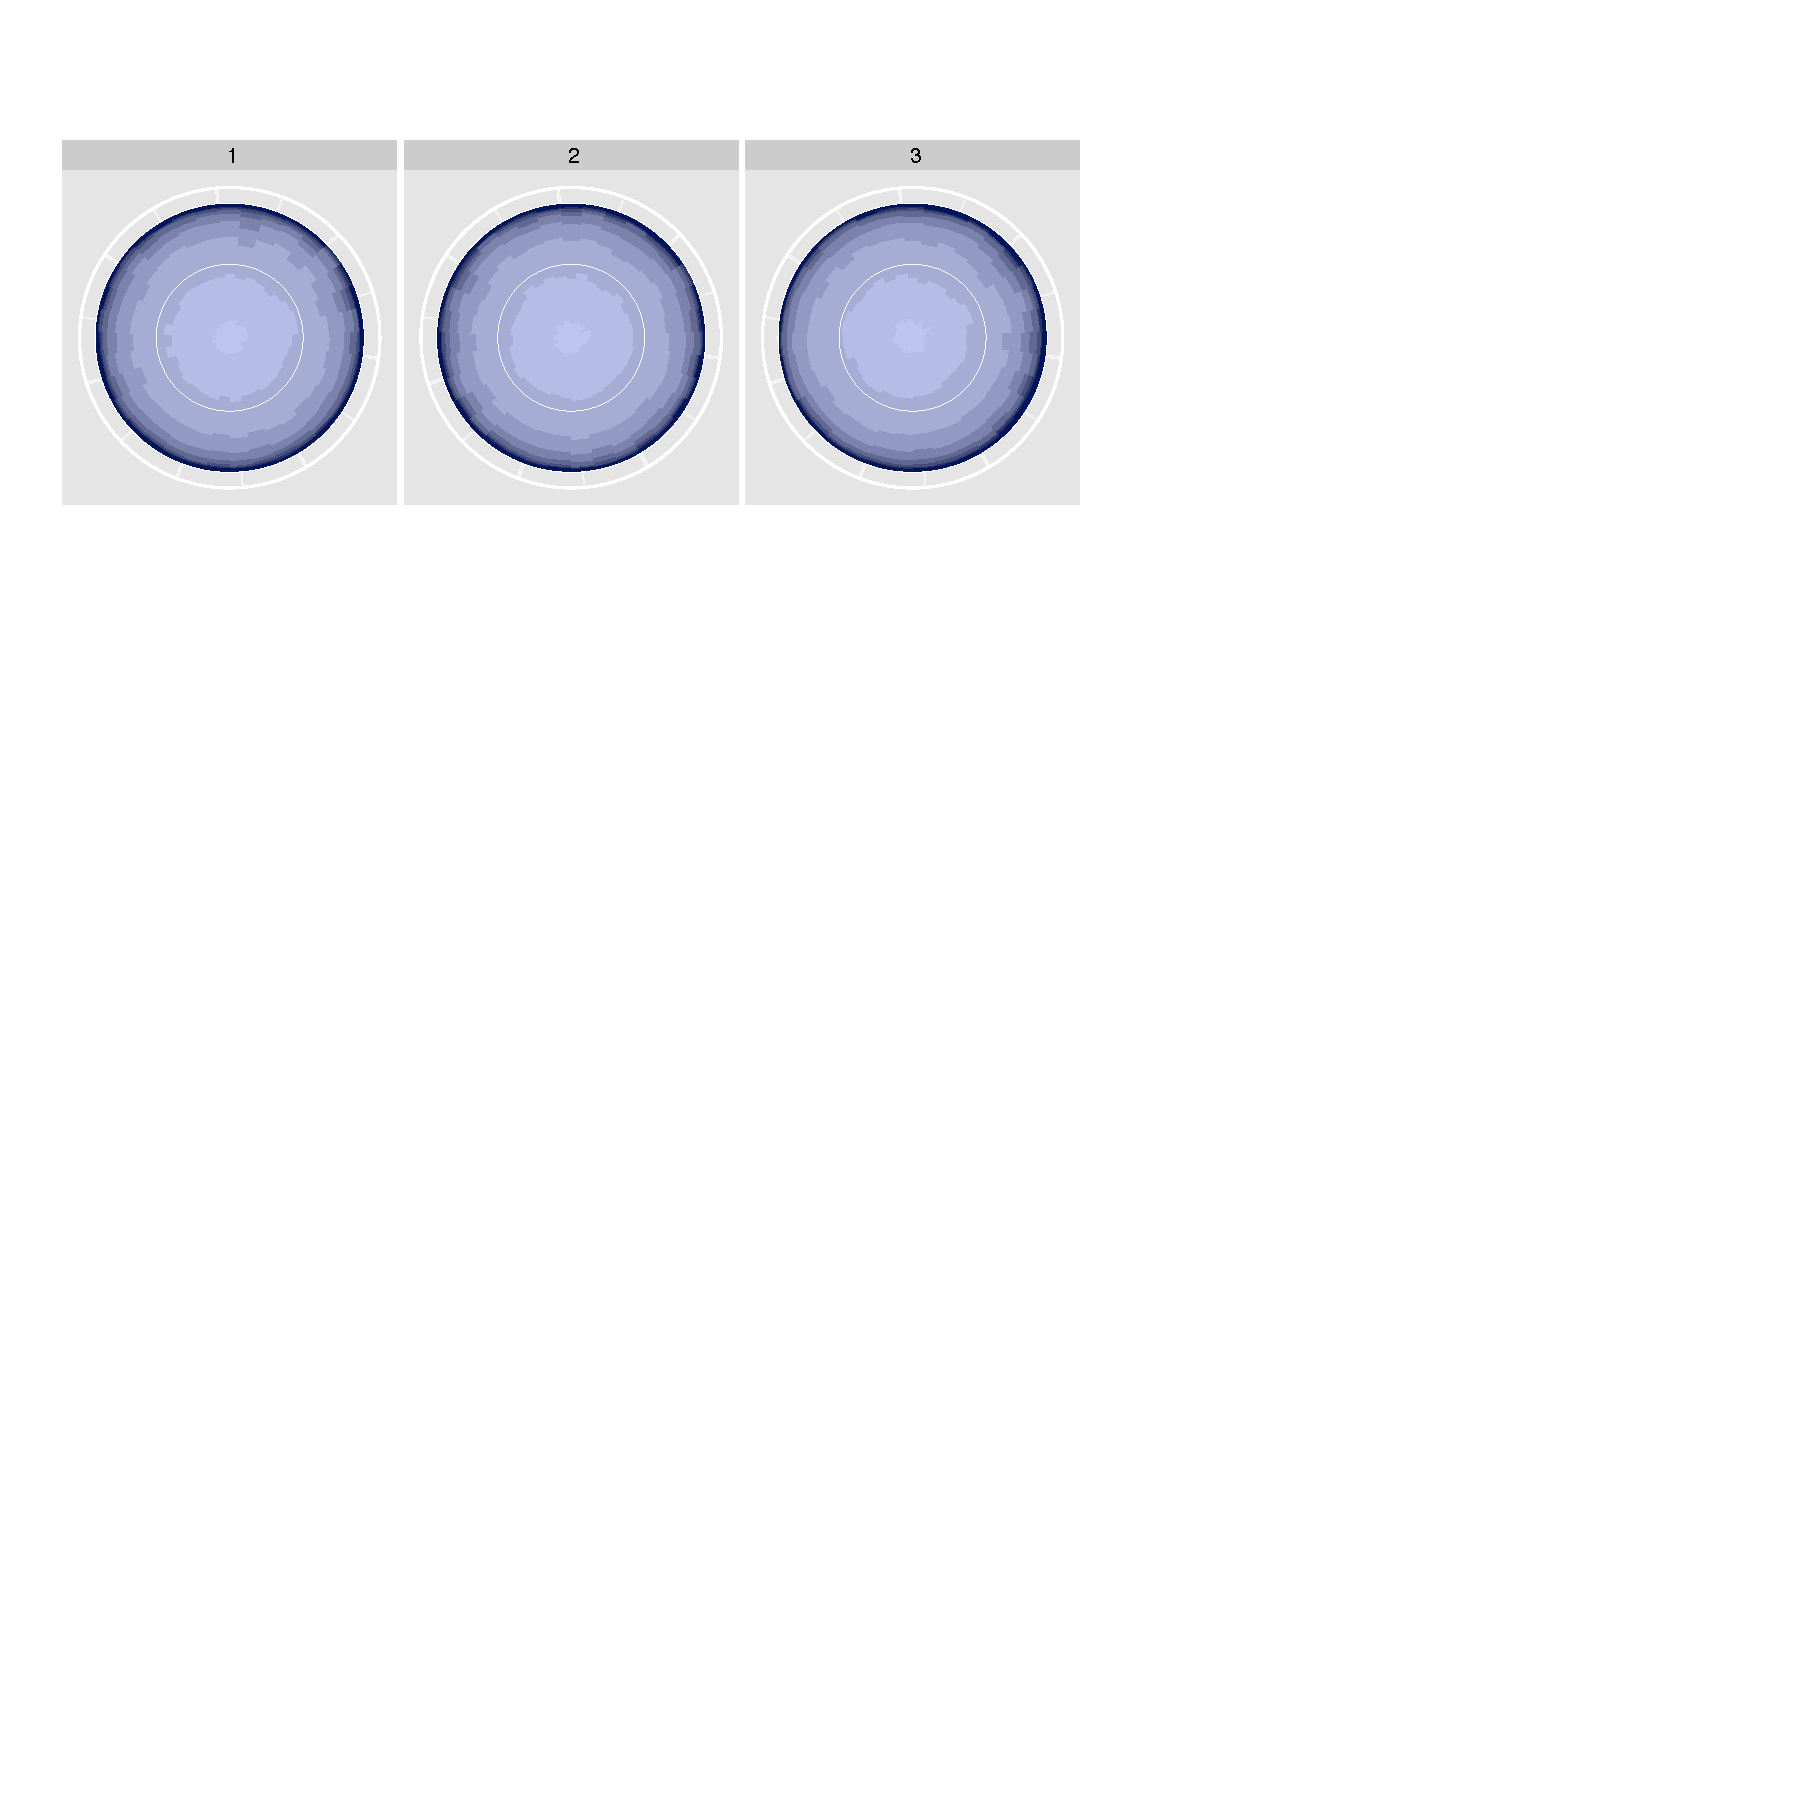
\includegraphics[height=1.2in]{polar}\hspace{0.05\linewidth}
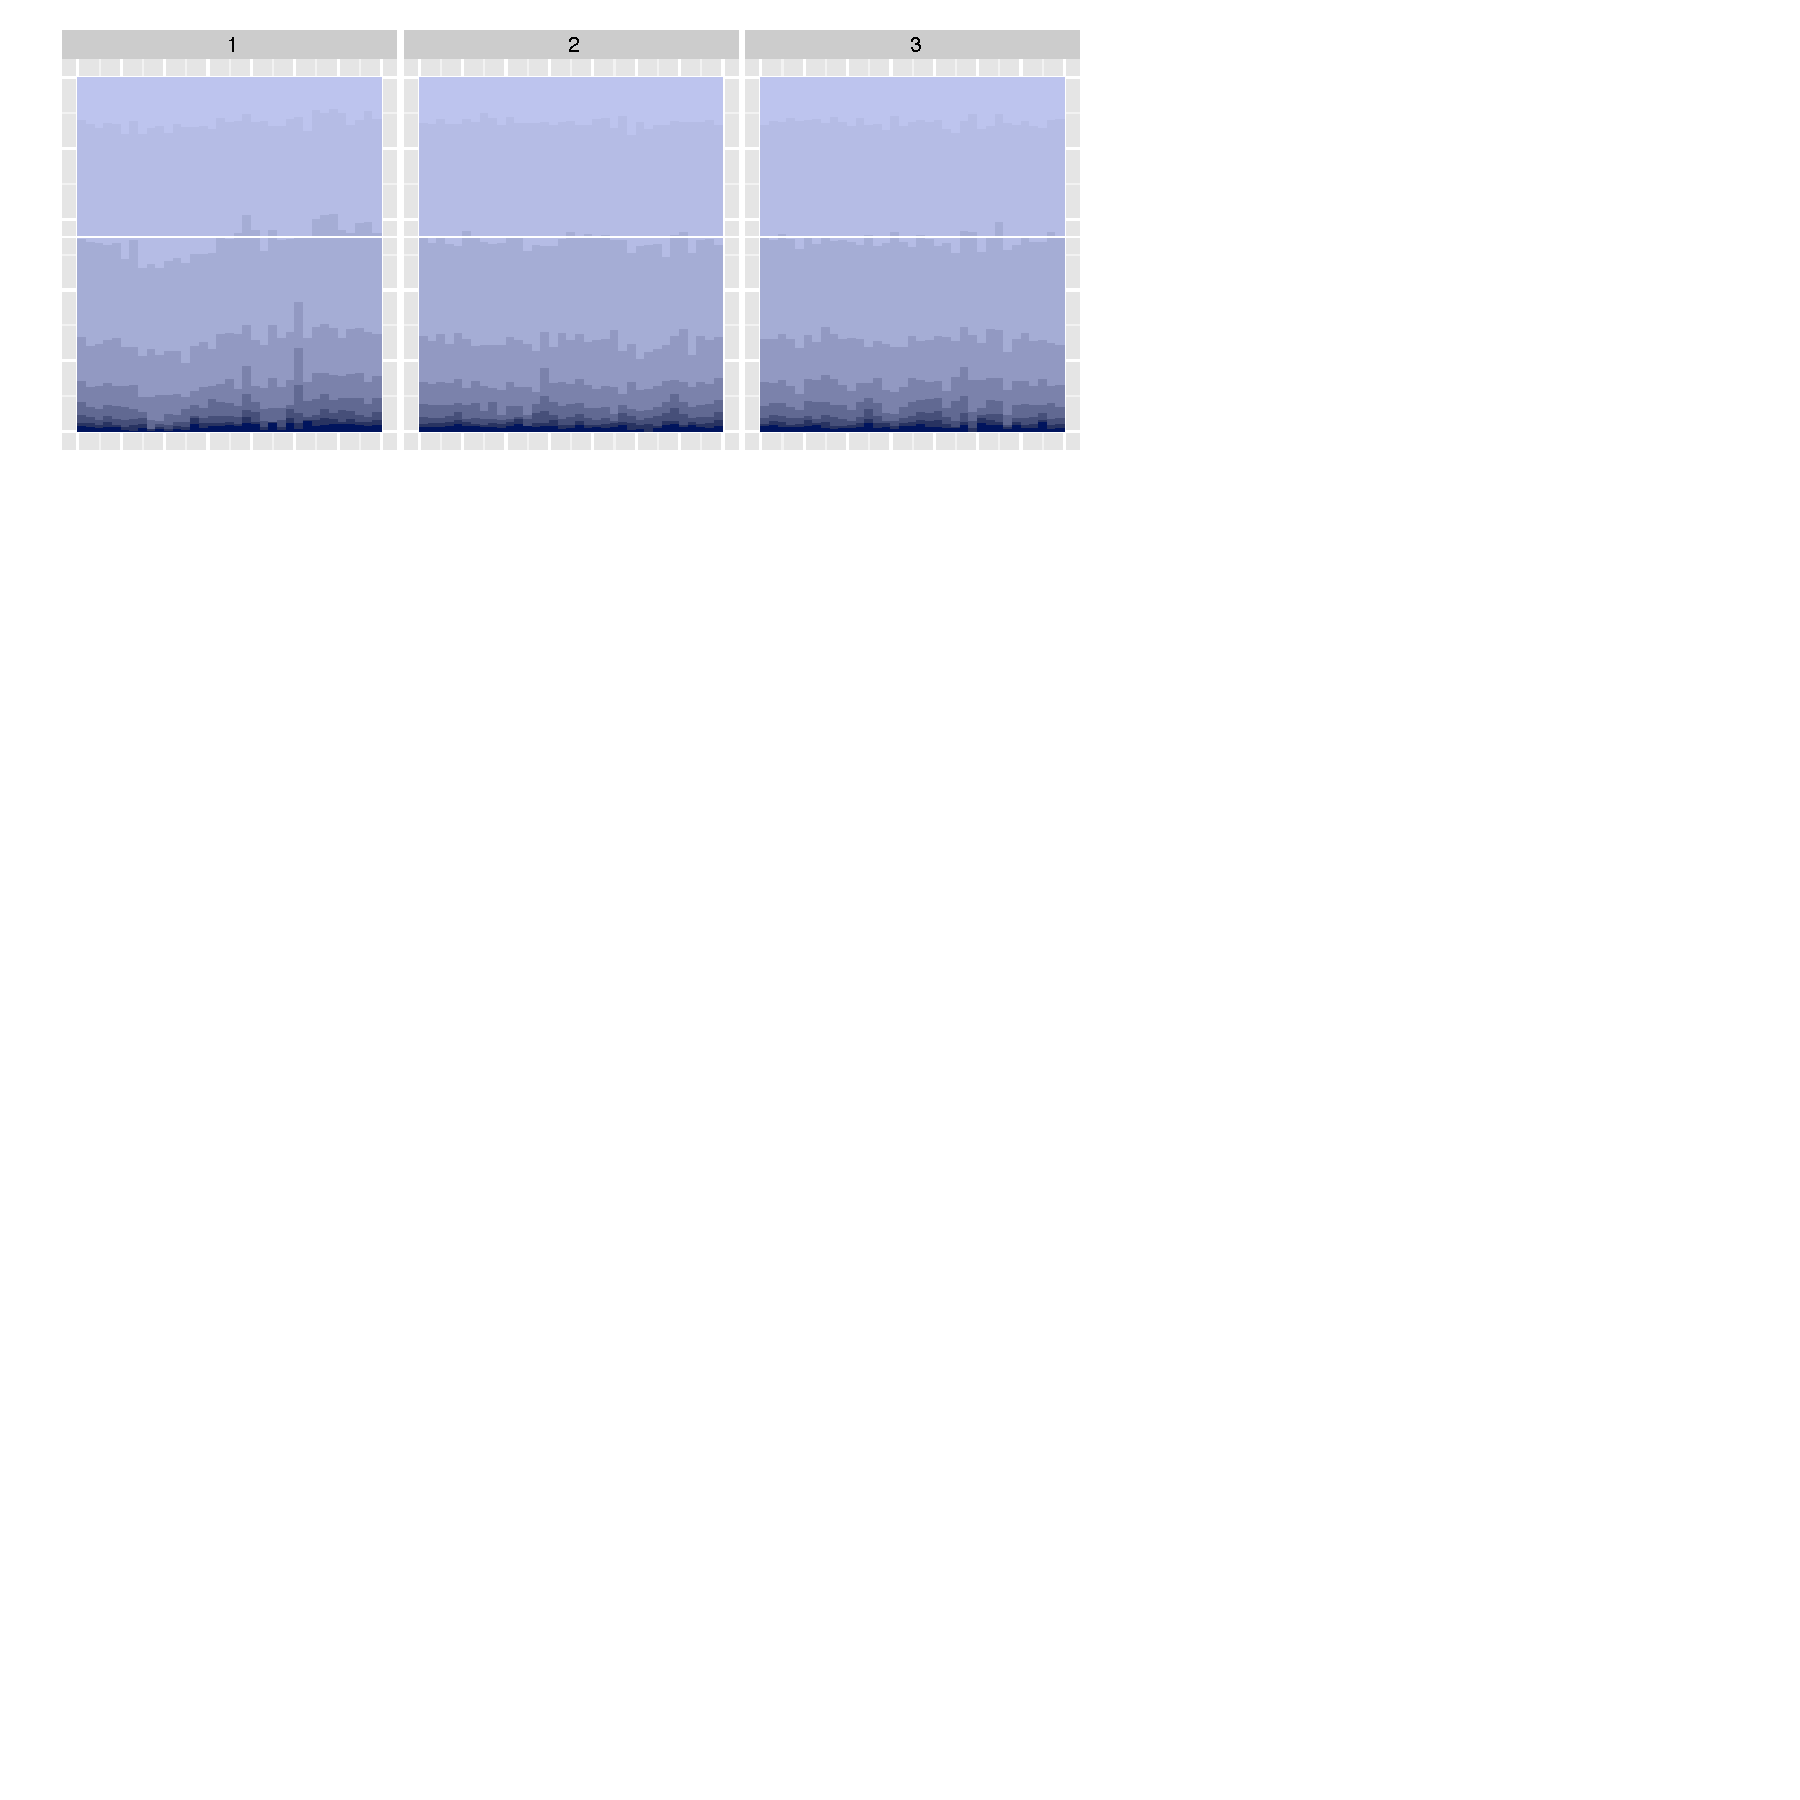
\includegraphics[height=1.2in]{eucline}
%\includegraphics[width=16cm]{CypressView.eps}
\caption{Which of the three plots is different from the others? - Is this question easier to answer with the Polar Charts or the Barcharts?}
}

%% Uncomment below to disable the manuscript note
%\renewcommand{\manuscriptnotetxt}{}

%% Copyright space is enabled by default as required by guidelines.
%% It is disabled by the 'review' option or via the following command:
% \nocopyrightspace

%%%%%%%%%%%%%%%%%%%%%%%%%%%%%%%%%%%%%%%%%%%%%%%%%%%%%%%%%%%%%%%%
%%%%%%%%%%%%%%%%%%%%%% START OF THE PAPER %%%%%%%%%%%%%%%%%%%%%%
%%%%%%%%%%%%%%%%%%%%%%%%%%%%%%%%%%%%%%%%%%%%%%%%%%%%%%%%%%%%%%%%%

\begin{document}

%% The ``\maketitle'' command must be the first command after the
%% ``\begin{document}'' command. It prepares and prints the title block.

%% the only exception to this rule is the \firstsection command
\firstsection{Introduction}

\maketitle

%% \section{Introduction} %for journal use above \firstsection{..} instead
%We introduce and discuss a tool for comparing different charts that are renderings of the same data in order to evaluate them for efficiency.
Graphics have a central role in the discovery process as well as in the presentation of results. 
As designer of  charts one of our main goals is to display data so that the information it contains is relayed in the most efficient way. 
In the search for the best display out of the seemingly endless multitude of methods we are guided by experience, knowledge of perceptual strengths and weaknesses, as well as aesthetic preferences. It is hard, if not impossible, to make the final decision on the design in an  objective manner. 
We can make this process less subjective by conducting user studies to evaluate competing designs of the same data, and measure designs for their efficiency by recordung how accurately and quickly viewers can extract pieces of information. 
User studies for evaluating different designs has a long standing tradition. For  statistical graphics user studies have their origin in the (convenience) study on evaluating difficulty of a set of different visual tasks by \citet{cleveland:1984}, which has recently been repeated finding similar results based on a larger and more representative study by \citet{kosara:2010}.

Usually, we need simulation studies to be able to completely control for the signal strength in the data. 
For charts, this is not a very realistic scenario. The need for displaying information particularly efficiently or accurately usually arises from  a particular problem while analyzing a data set, from which we want to learn new insight. Often, it is difficult to simulate data in such a way that it realistically represents the particular problem, which in turn makes it dubious whether the results from a simulation study are actually applicable to the problem at hand, reminding us painfully of George Box's famous quote on models: ``essentially, all models are wrong, but some are useful." \citep[page=424]{box}  

Lineup tests  \citep{buja:2009} allow us to directly use the data at hand to evaluate different competing designs by using permutations tests \cite{good:2011} of the original dataset. We can therefore get valid quantitative measures for comparing different designs without having to set up a simulation.

When we are presenting a chart we  want to convince our audience of the presence of a particular feature or relationship in the data. 
In order to enable us to draw a conclusion about presence or absence of a feature in the data, we have, however, to assess what features show up based purely on marginal distributions rather than joint distributions.

\begin{figure}[htbp] %  figure placement: here, top, bottom, or page
   \centering
   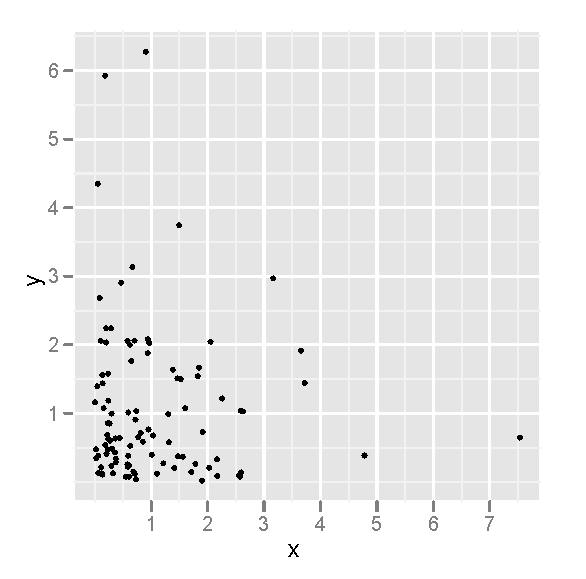
\includegraphics[height=0.32\linewidth]{rexp.pdf} 
   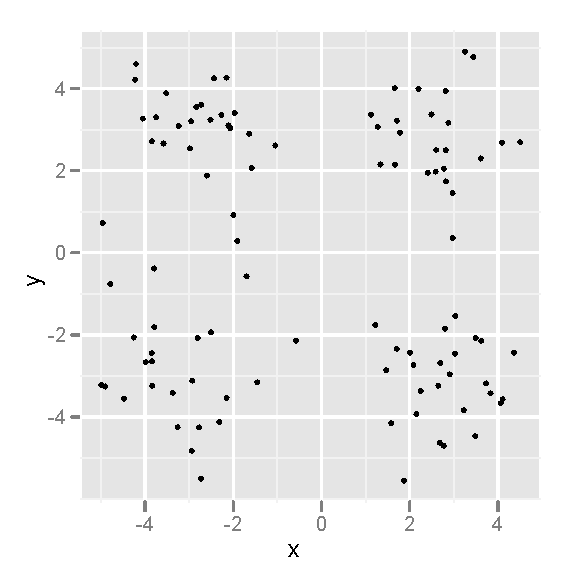
\includegraphics[height=0.32\linewidth]{rnorm.pdf} 
   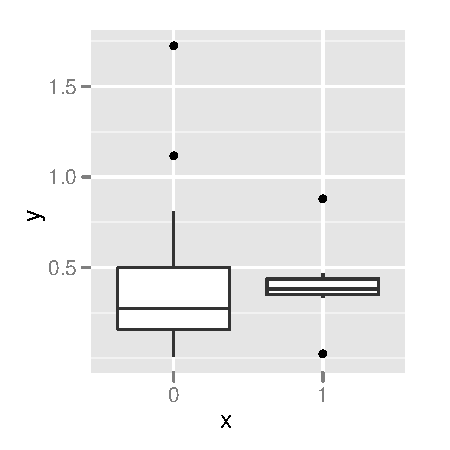
\includegraphics[height=0.32\linewidth]{two-exp.pdf} 
   \caption{Examples of charts with distinctive features but independent variables. From left to right: scatterplot of $X$ and $Y$ with independent $X, Y \sim Exp_{\lambda=1}$; scatterplot of two variables with mixed normal distribution $N(3,1)$ and $N(-3,1)$; boxplot of $X$ and $Y$ with $X \sim B_{n=100, p=0.1}$ and $Y \sim Exp_{\lambda=1}$. }
   \label{random}
\end{figure}

Features in the marginal distributions, such as multi-modality, skewness  or outliers, might interfere with our intuition of what `randomness' might mean in a particular situation and lead us to wrong conclusions. All of the plots in figure \ref{random} show distinctive features. None, of these, however, is a feature of the joint distribution, i.e. all of the variables involved are independent of each other. The scatterplot on the left of figure \ref{random} shows data sampled from an exponential distribution with rate parameter $\lambda=1$. The data in the middle comes from mixing two normal distributions with different means: half of the points has mean $\mu_1 = -3$, the other half has mean $\mu_2=3$, which results in the distinctive four groups.
The two boxplots on the right appear to show a median shift between the two groups. This, however is a result of both the group size (only 7\% of the points is in the second group) and a skew distribution in vertical direction, with $y \sim Exp_{\lambda=1}$. 


Lineup plots have been shown as an effective tool \cite{wickham:2010} for enabling us to quantitively assess the strength of the relationship between $X$ and $Y$.
In a lineup plot the plot of the actual data is -- as in a police line-up -- inserted among decoy plots. The decoy or {\it null} plots are generated in a way that is consistent with the null hypothesis, i.e. these are plots in which we can assume that any relationship visible is there purely by chance. This gives us a reference framework against which to compare the data plot and, if we are still able to identify the data plot from the lineup because of a distinguishing feature, we have formal evidence that the feature in the data is, in fact, not just coincidental. 

The strength of this evidence is determined by both the number of independent evaluations as well as the size of the lineup. (XXXX needs more motivation HH) The signal strength \cite{majumder:2011} of a particular lineup is given as:
\[
\text{signal strength} = 1- \left( \frac{x}{n}\right)^{1/(m-1)},
\]
where $m$ is the size of  the lineup, i.e. the number of individuals shown, and $x/n$ is the ratio of correctly identified data plots ($x$) in  $n$ independent evaluations. Signal strength is limited to a range of values between 0 and 1. Higher values indicate stronger signal.
 In the case of a parametric situation (i.e. the feature shown in the chart can be described in parametric form as a real-valued vector $\theta$ in the data), the signal strength is equivalent to the statistical power of the test.

\section{Lineups for Comparing Designs}
We are going to make use of the signal strength gained from multiple viewings of a lineup in order to evaluate competing designs as follows:
\begin{enumerate}
\item{{\bf Create Lineup Data:} create $m-1$ permutations of $y$}
\item{{\bf Create lineups from competing designs:} use the same data}
\item{{\bf Evaluate Lineups:} assess both signal strength and time taken by individuals to come to a decision.}
\item{{\bf Evaluate Competing Designs:} differences in signal strength or time to decision are due to differences in the design. In the case of multiple observations for each individual, we can also correct for an individual's visual ability. }
\end{enumerate}

XXXX should we include nullabor code?

%We also know that humans learn about new information through a visual search pattern that emphasizes new information (Wolfe, 2002; Rensick, et al., 1997). Of course, the type of visualization should take the natural human inclinations into account as well. For instance, a good visualization will account for both the �gestalt? like perceptual tendencies as well as the detail-orientated nature of cognition (Kosslyn, Thompson and Ganis, 2002; Pylshyn,2003)


% !TEX root = comparison.tex
\section{Experimental Setup}
We want two discuss two applications, in which we are making use of lineups to compare competing designs. 
The first one arises from a discussion of how wind direction affects efficiency of an airport. In this example, we are dealing with all flights \cite{rita} in and out of Seattle/Tacoma International Airport (SEA) between July 2008 and June 2011. As a measure of airport efficiency we are using time between successive wheel-events (time at wheel take-off or touch-down), which we found to be independent of airline carrier and operating hours, as long as we restricted the data to `regular' operating hours between 7 am and midnight and `regular' weather conditions -- i.e. we eliminated records associated with the top 5\% wind speed measurements \cite{noaa-weather}, leaving us with just under 0.5 Million flights.

Statistical tests of mean efficiency by wind direction are not particularly helpful in this situation:
the difference in mean efficiency between the most efficient wind direction and the least efficient shows a statistically significant difference with a $p$-value $\le 10^{15}$. %2.2e-16$. 
However, out of the 34 other wind directions,  another 31 show significant differences in efficiency as well. This is much more a property of the large data size rather than practically usable differences. Mere significances also do not allow us an assessment of the underlying pattern.

\subsection{Wind Direction and Airport Efficiency}
In deciding on the design for displaying efficiency  by wind direction we were using the fact that wind direction is circular, and  displayed the data as (conditional) wind rose charts - i.e. for each of 36 wind directions we show the percentage of flights falling into one-minute intervals between successive flights, from  0 minutes to 8 minutes or more.


\begin{figure}[htbp] %  figure placement: here, top, bottom, or page
%   \centering
 \hspace{-.1in}
   \begin{tabular}{ccl}
   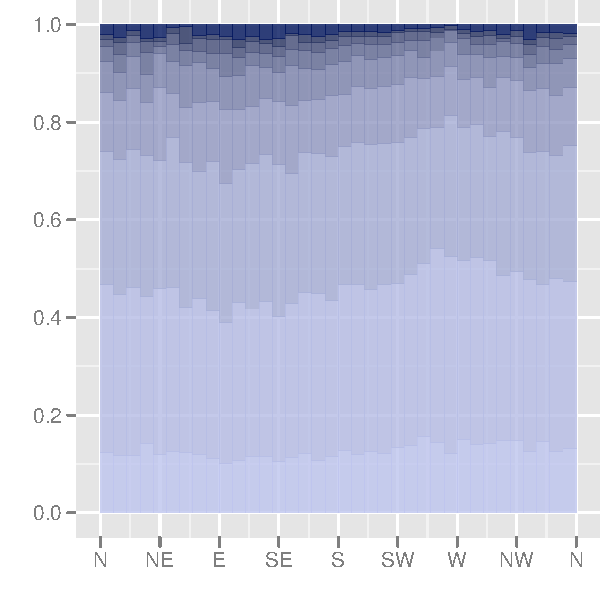
\includegraphics[width=0.375\linewidth]{euclid_noline.pdf} & \hspace{-.3in}
   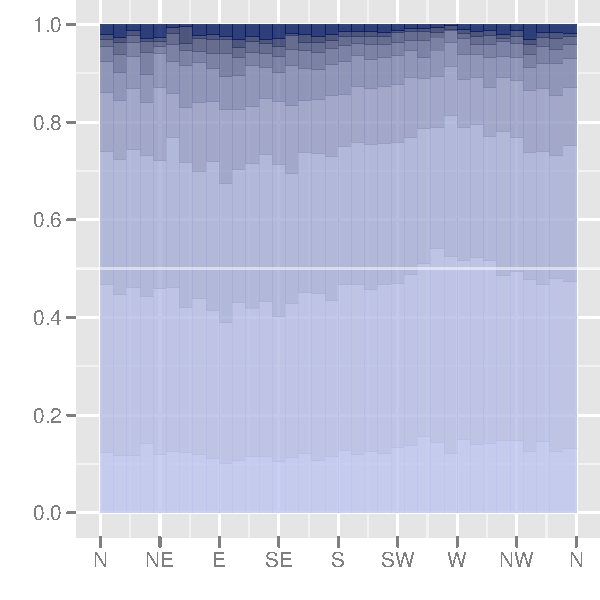
\includegraphics[width=0.375\linewidth]{euclid_line.pdf} &  \hspace{-.2in} \multirow{2}{*}[.55in]{  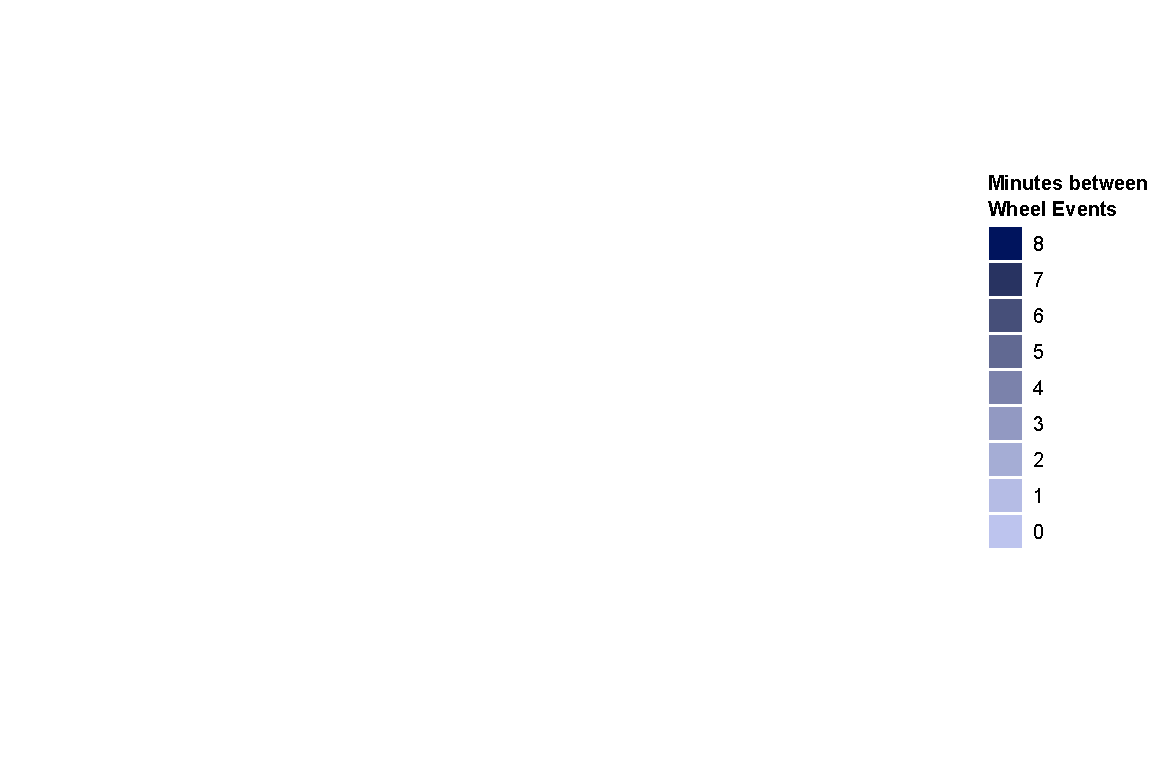
\includegraphics[width=0.2\linewidth]{legend.pdf}} \\
   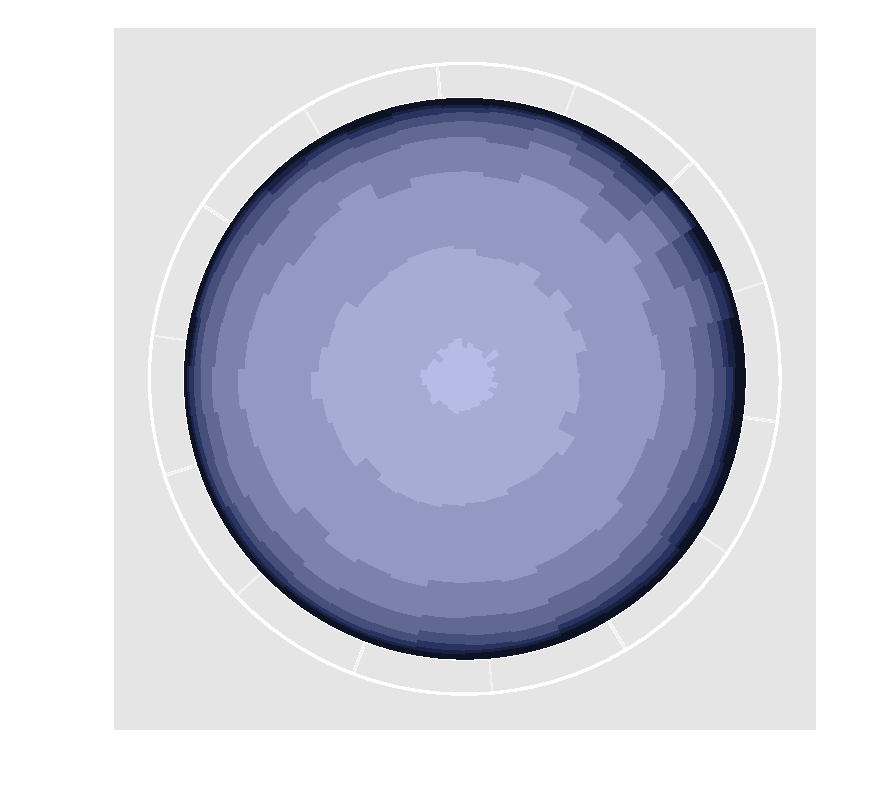
\includegraphics[width=0.43\linewidth]{Polar_NoLine.pdf} &  \hspace{-.3in}
   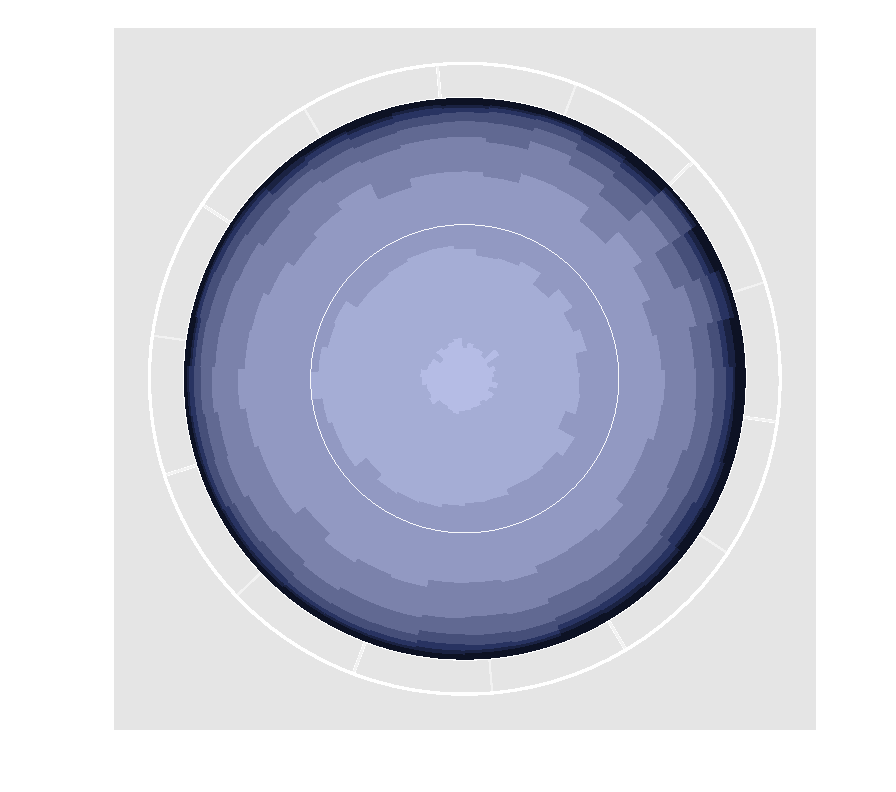
\includegraphics[width=0.43\linewidth]{Polar_Line.pdf}  
   \end{tabular}
   \caption{All four competing designs: polar versus Euclidean charts in top and bottom row, with (right) and without (left) reference lines at 50\%. }
   \label{layouts}
\end{figure}

In spite of the contextual circular property of wind direction, the pattern in efficiency did not seem to stand out well during the exploration process, which led us to using a corresponding  Euclidean design. Both designs were additionally equipped with a reference line at 50\%. 
Figure \ref{layouts} shows an overview of all four chart types in the study. During the exploration of the data, it became clear that Seattle airport functions at it best with winds coming from the East to Southeast, while winds from the West seemed to be most troublesome, resulting in a wave-like pattern in the Euclidean charts and a shift in center for the polar charts. Since runways can be used in both directions, changing the runway usage according to dominant wind direction for that day or time of the year might be a feasible solution in gaining efficiency. 

\begin{figure}[htbp] %  figure placement: here, top, bottom, or page
   \centering

\begin{tabular}{cl}
\phantom{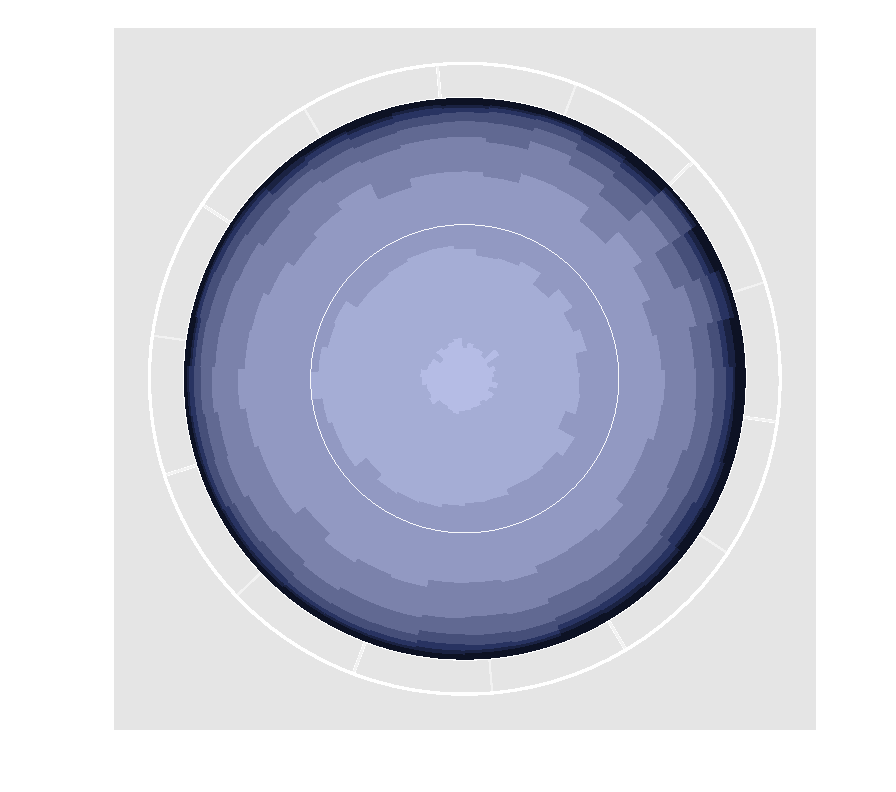
\includegraphics[width=0.03\linewidth]{Polar_Line.pdf}} & \vspace{-0.035in} \multirow{10}{*}{\hspace{-0.25in}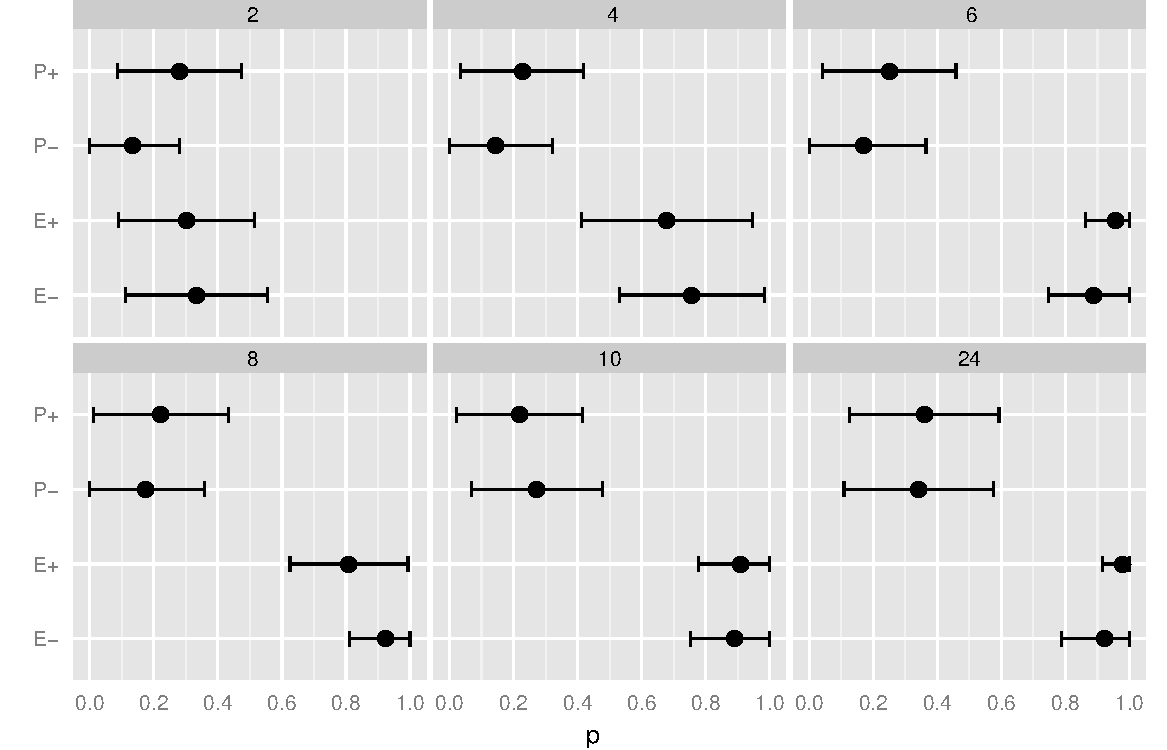
\includegraphics[width=0.9\linewidth]{turk4-designs.pdf}} \\
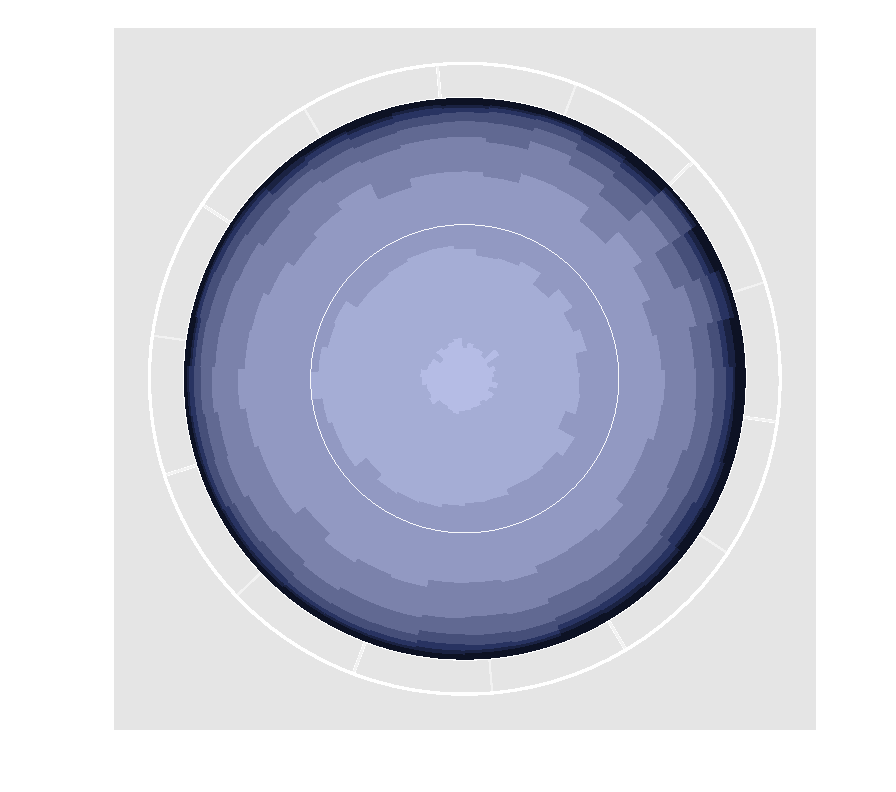
\includegraphics[width=0.05\linewidth]{Polar_Line.pdf} \\
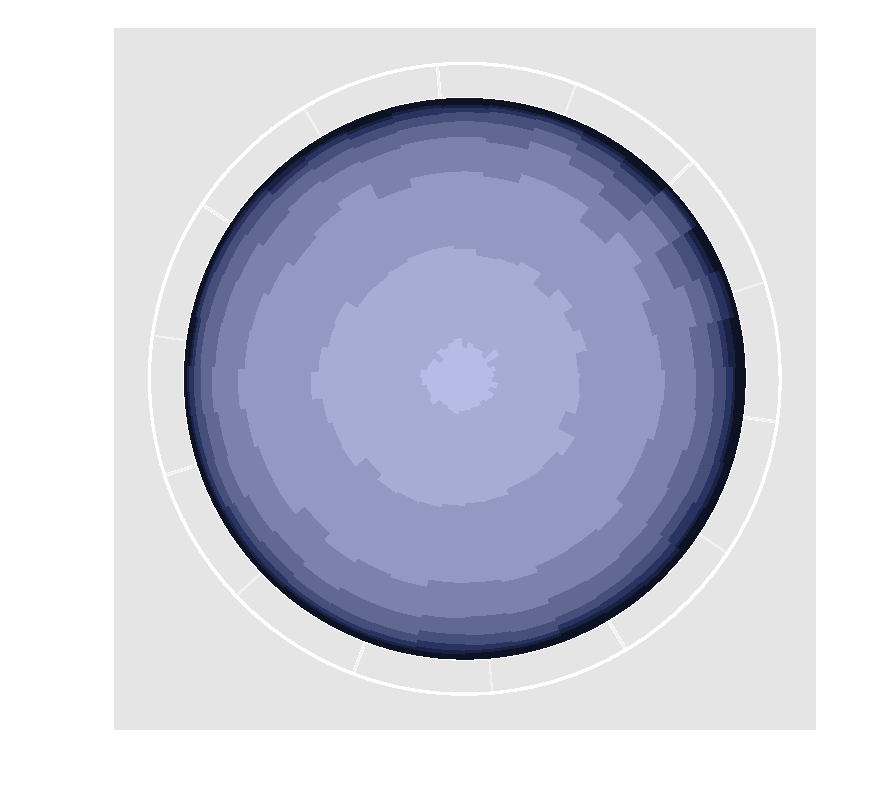
\includegraphics[width=0.05\linewidth]{Polar_NoLine.pdf} \\
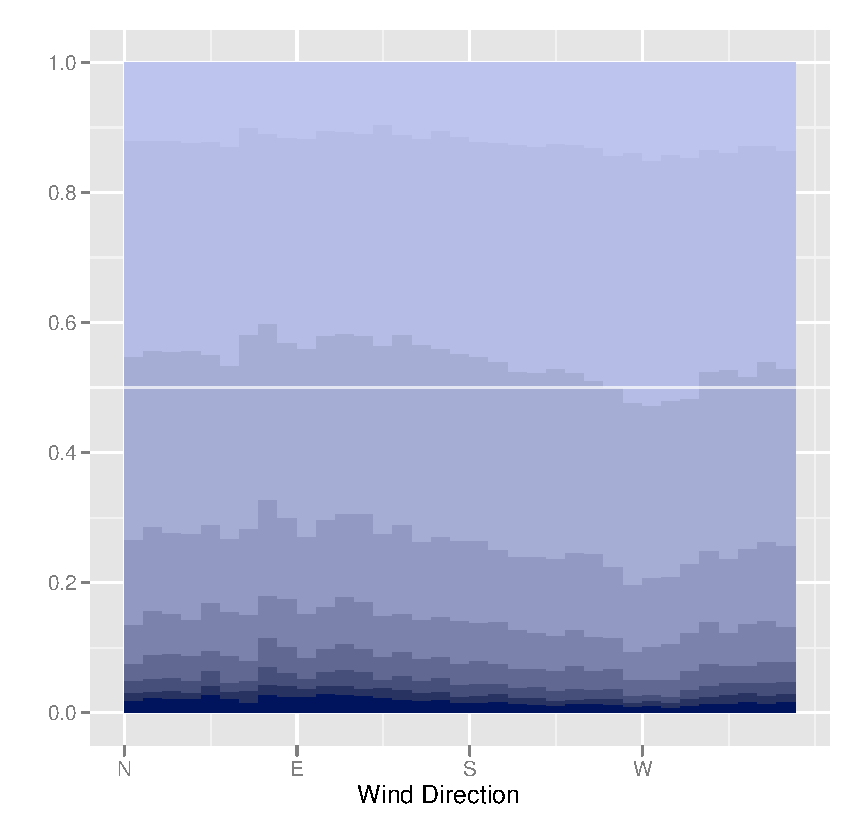
\includegraphics[width=0.043\linewidth]{Euclidian_Line.pdf} \\
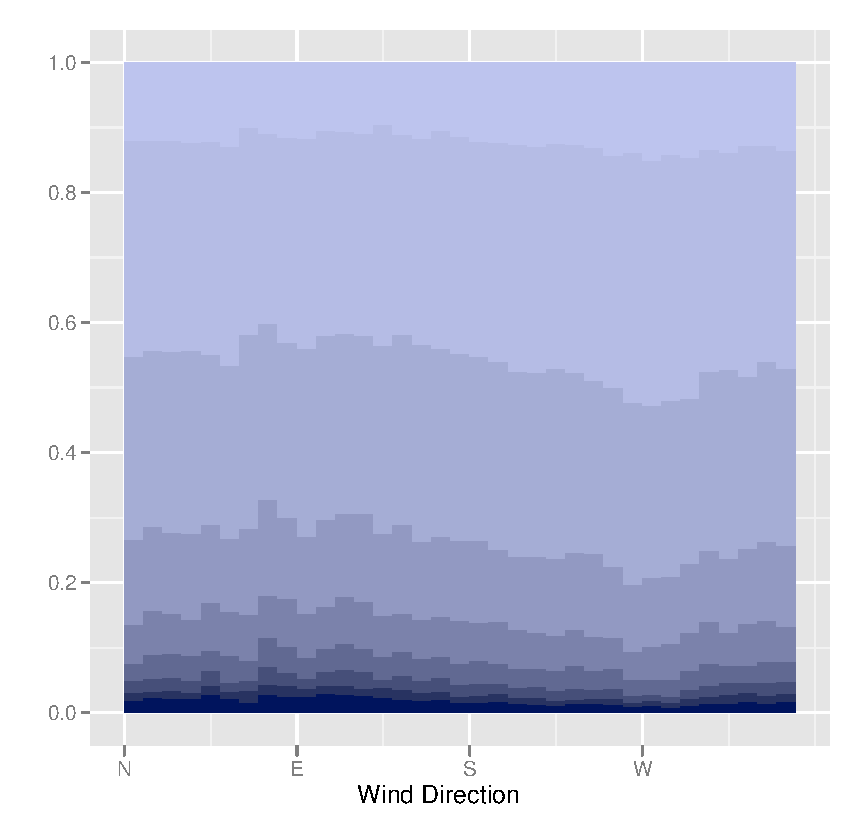
\includegraphics[width=0.043\linewidth]{Euclidian_NoLine.pdf}\\
\phantom{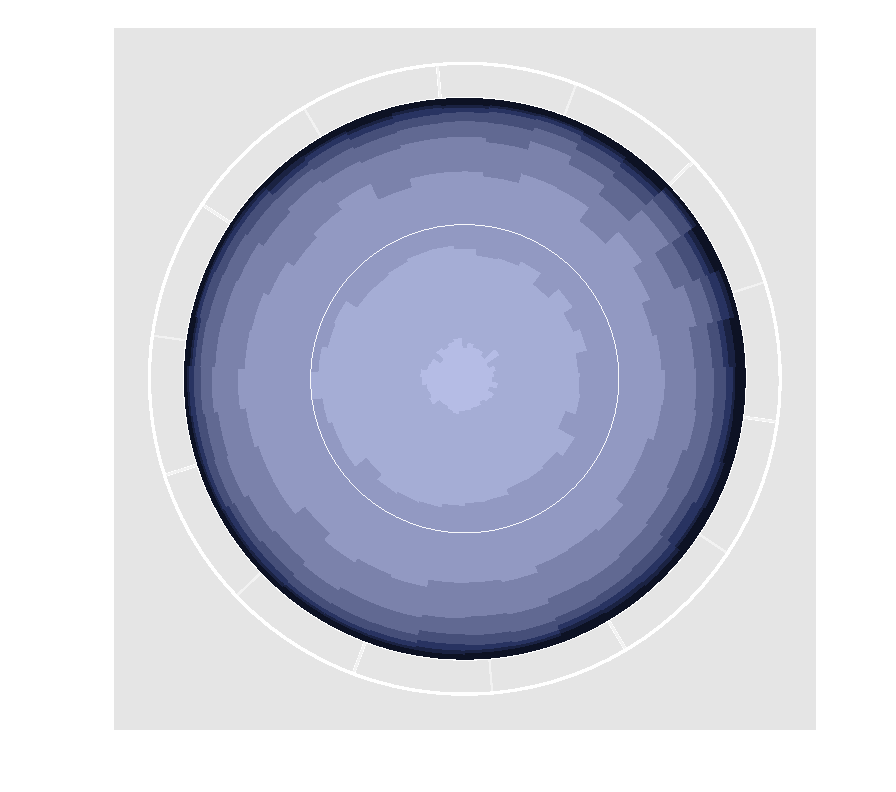
\includegraphics[width=0.015\linewidth]{Polar_Line.pdf}}\\
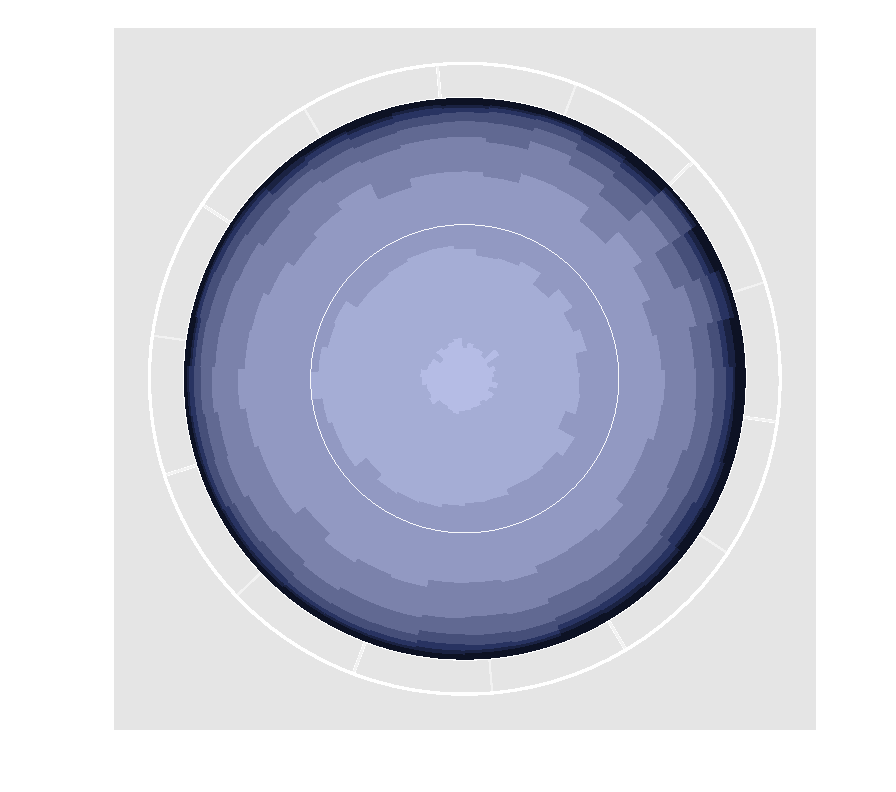
\includegraphics[width=0.05\linewidth]{Polar_Line.pdf} \\
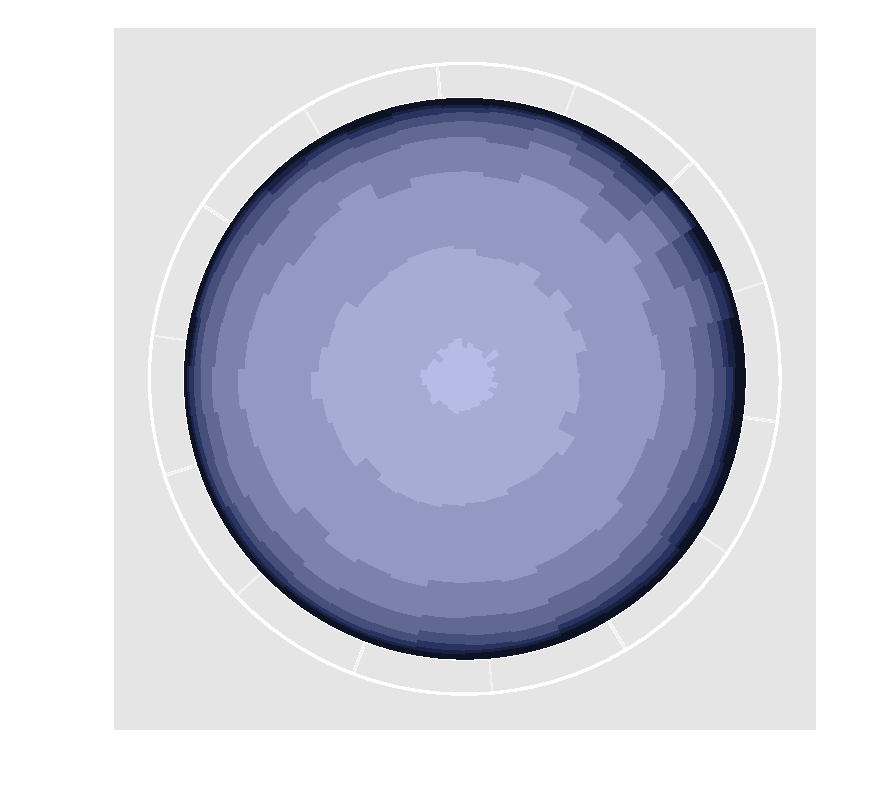
\includegraphics[width=0.05\linewidth]{Polar_NoLine.pdf} \\
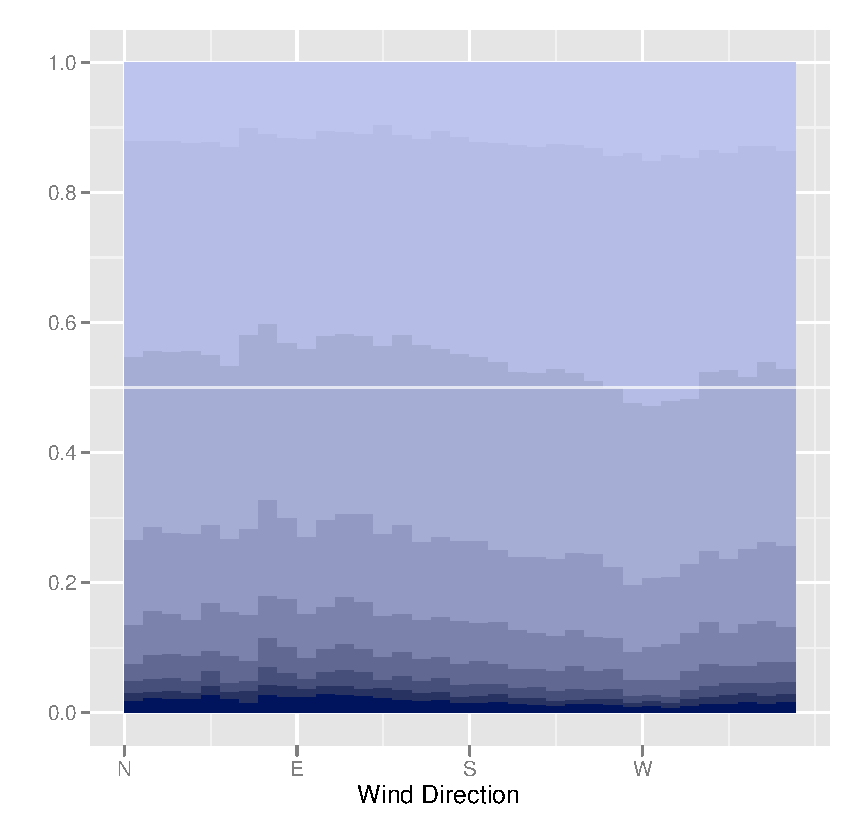
\includegraphics[width=0.043\linewidth]{Euclidian_Line.pdf} \\
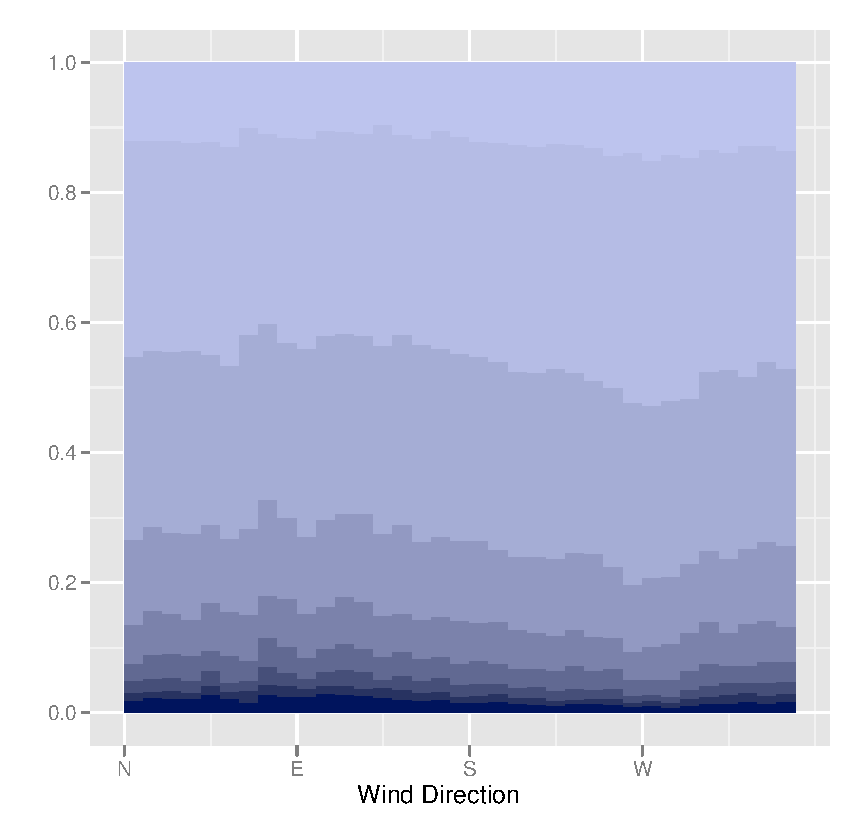
\includegraphics[width=0.043\linewidth]{Euclidian_NoLine.pdf}\\
  \end{tabular} 
  \vspace{0.1in}
   \caption{Power results for two competing designs: polar versus a Euclidean, with and without a reference line. Error bars indicate 95\% confidence intervals. Plots are facetted by percentage of data used. }
   \label{fig:treatment}
\end{figure}

An additional factor we were interested in this particular situation was to assess, how much of the data we actually needed to use in a design to have observers pick out the pattern. Clearly, a design is more efficient, if a smaller sample size is sufficient for showing the presence of a relationship. In order to investigate this, we took different size samples of the data and created lineup plots of all four designs for these subsets. The effect of sampling size on the displays mostly stems from the additional variability introduced when using small samples, which might hide the pattern, if it is not displayed prominently. 
XXX picture of sampling size?
Another perturbation to the data are `shifts' in wind direction, i.e. we make use of the circular nature of the wind direction and adjust the $x$ axis by using different offsets.

\begin{figure}[htbp] %  figure placement: here, top, bottom, or page
   \centering
   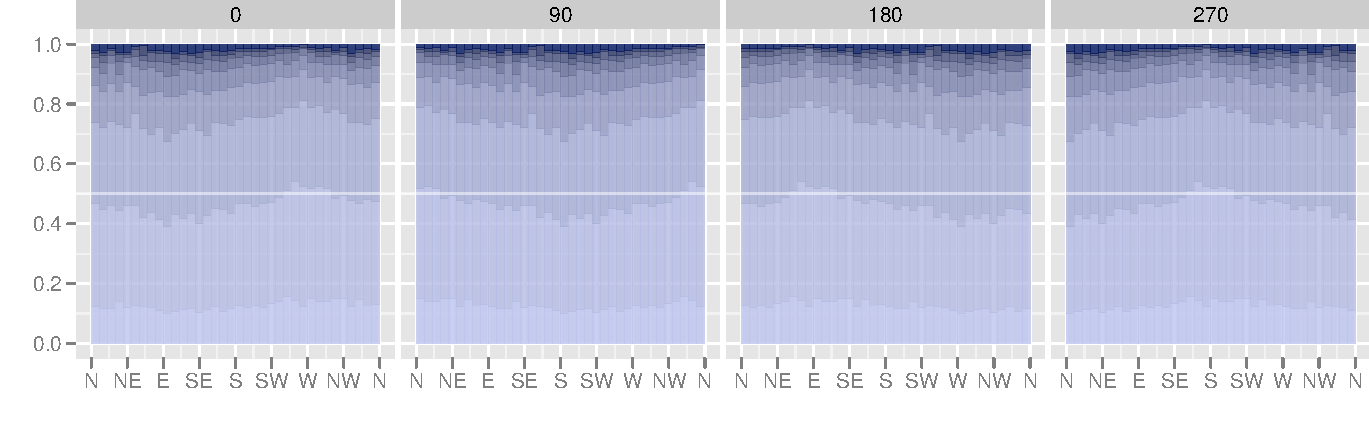
\includegraphics[width=\linewidth]{euclid-offset} 
   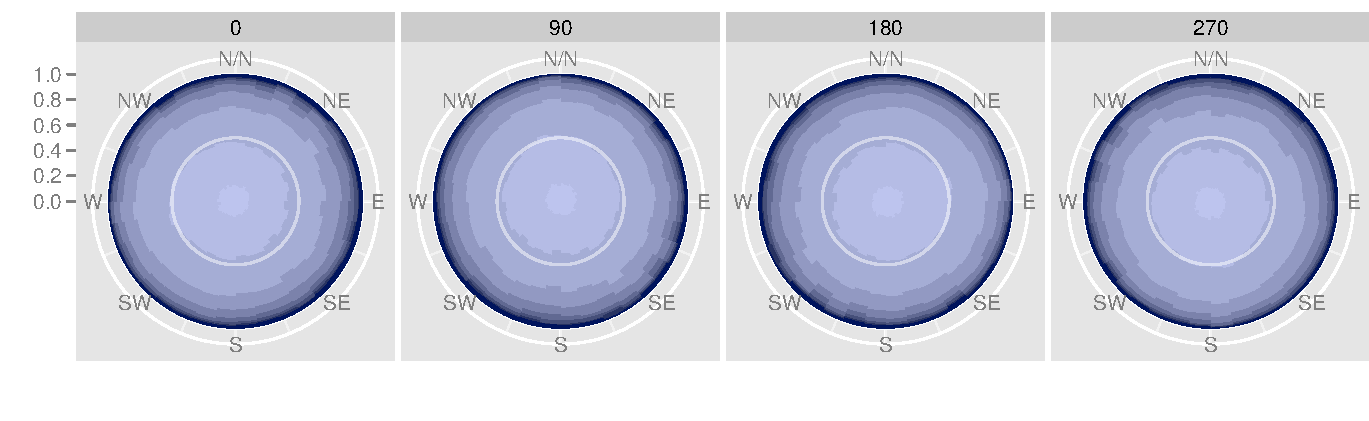
\includegraphics[width=\linewidth]{polar-offset} 
   \caption{ \label{fig:offset} (Top) Euclidean charts of the same sample, with shifts in wind direction by 90, 180, and 270 degrees. The shift by 90 and 270 leads to a `valley' versus a `mountain' pattern, whereas a shift by 180 degrees inverts the wave pattern from `down-up' to `up-down'.\hfill\newline
      (Bottom) Shifts in wind direction in the polar chart lead to rotations of the display by 90 degrees.}
\end{figure}

 This results in a shift of the wave in Euclidean charts and a rotation in the polar charts as can be seen in figure \ref{fig:offset}. Our initial hypothesis was that this would have no effect on the polar charts, but might have a deteriorating effect on the Euclidean charts, in the case that the peak or the valley of the wave was at either end of the $x$ axis. 
While these simple perturbations and different sample sizes allow us to get insight into different aspects of the designs, they also allow us to get multiple responses from each observer to assess individual ability without the need to go outside the framework of the original data, i.e. we leave the joint relationship between $x$ and $y$ essentially unchanged. For all of these combinations we produced two replicates, resulting in a total of 192 different lineups ($ 4 \text{ designs} \times 6 \text{ sample sizes} \times 4 \text{ offsets} \times 2 \text{ reps})$.

Data was collected using Amazon's Mechanical Turk (MTurk) service. XXX More details: website and screen shot.
 Each participant was shown ten lineups. In order to avoid people `gaming the system' as found in earlier studies \cite{heer:2010, kosara:2010}, participants were shown two specially prepared lineups as a baseline of performance -- if participants got just one of these two reference lineups correct, we required at least an overall correct percentage of 20\%, which is indicative of a performance that is better than guessing. Table \ref{tbl:treatment} gives an overview of the number of times lineups in each combination of design and sample size were shown, and in how many of them the data plot was correctly identified. 

\begin{table}[hbtp]
\resizebox{\linewidth}{!} {
	\rowcolors{1}{white}{lightgray}
	\begin{tabular}{ll|@{}r|@{}r|@{}r|@{}r|@{}r|@{}r}
	\multicolumn{2}{l}{sample size (in percent)}  & 2 & 4 & 6 & 8 & 10 & 24 \\ [1pt] \hline
	Polar & with & 13/49& 9/43 & 9/39 & 7/35 & 8/40 & 13/38 \\
	& without & 6/51&   4/34 &  5/34 &  6/39 & 11/43 &  12/37\\ [1pt] \hline
	Euclidean & with &12/24& 18/27 & 42/44 & 33/41 & 39/43 & 46/47\\
	& without & 13/41 &24/32& 39/44 & 47/51 & 40/45 & 34/37\\
	\end{tabular}
	}
\caption{\label{tbl:treatment} Breakdown of lineups: correct/shown. Each participant was shown eight lineups from the set above and two separate `test' charts.}
\end{table}

Besides correctness of responses, two additional response variables were recorded:  time taken for answer and a (subjective) confidence level, ranging from 1 (lowest) to 5 (highest), assessing how convinced participants are of the correctness of their answer. 
Figure \ref{fig:time} shows time taken until a decision was made in histograms, facetted by design and colored by correctness of answer. because of the skewness of the distributions, times were log-transformed. Polar charts take on average more time to answer, but are answered with much lower precision. Figure \ref{fig:conf} shows two barcharts of confidence levels by task, again coloring is used for correctness of answers. Euclidean displays lead to a very bimodal distribution of confidence: participants are either very sure or not sure at all of their answer. Confidence levels in polar charts are distributed much more uniformly.

\begin{figure}[htbp] %  figure placement: here, top, bottom, or page
   \centering
   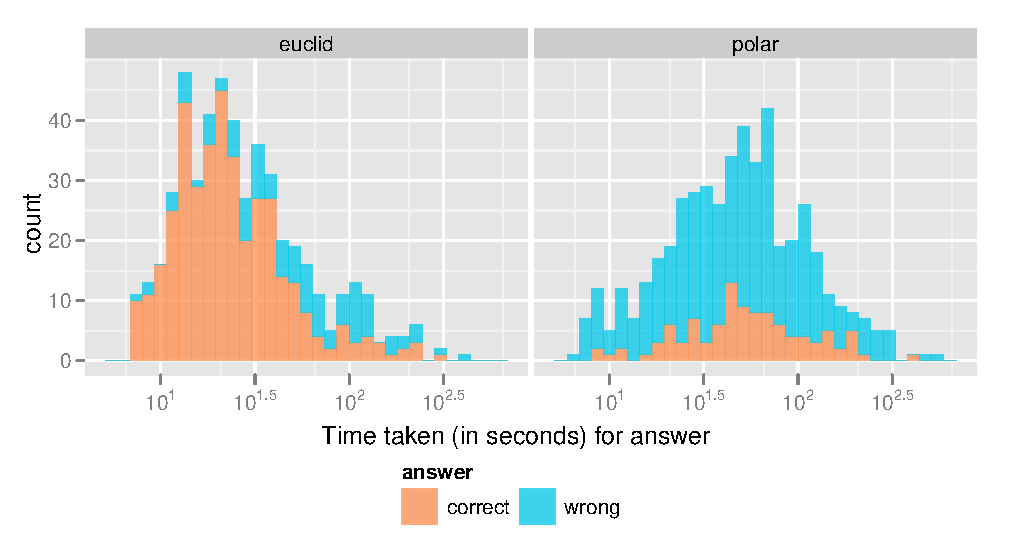
\includegraphics[width=\linewidth]{time-answer} 
   \caption{Histograms of time taken for answering lineups. On average the Euclidean design is answered faster and with higher power (percentage of correct answers). }
   \label{fig:time}
\end{figure}

\begin{figure}[htbp] %  figure placement: here, top, bottom, or page
   \centering
   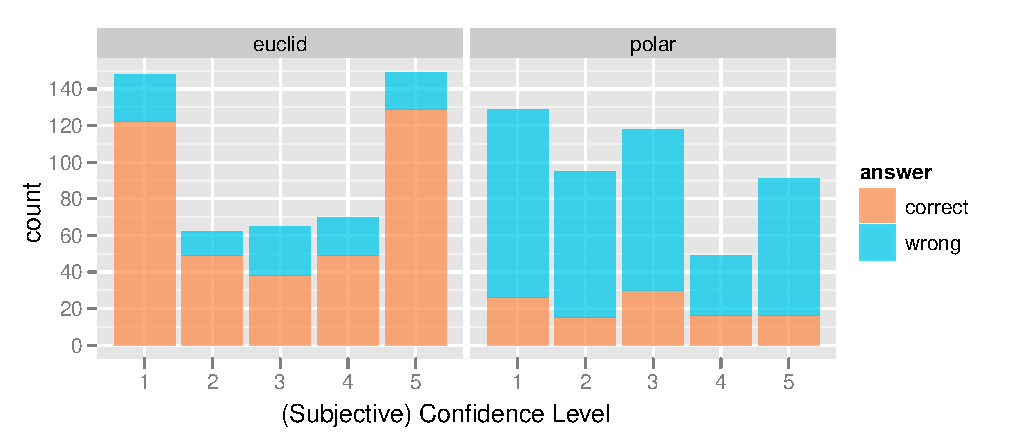
\includegraphics[width=\linewidth]{conf-answer} 
   \caption{Barcharts of (subjective) confidence in answering correctly for each lineup. A strongly bimodal distribution is apparent, while confidence levels for polar charts are more uniform. There are only slight (and non significant) difference between confidence levels and correctness of results.}
   \label{fig:time}
\end{figure}


Most generally this experiment can be paralleled to the pie chart versus barchart discussion \cite{***}. 
The Euclidean coordinate plot is made up of bars where areas are colored proportionally according to percentages. The polar coordinate plot is made up of pie slices which are also colored proportionally according to the data. 
Viewers of these charts will visually decode the areas of the bars and pie slices and make a judgement based on their decoding. According to  \citet[page=40]{kosslyn:2006}, area is usually perceived as a function of what the actual area is. This function is the area raised to an exponent of approximately 0.8 and then multiplied by a constant. However, when bars are parallel, the relative height of these bars is perceived very accurately. From this information, one could infer that the Euclidean coordinate plot may gain efficiency based on the height of the colored bars. 


For evaluating the results, we are using a linear mixed effects modeling \cite{pinheiro:2000} approach in all three of our response values, using the {\t R} package {\tt lme4} \cite{bates:2011}. 


Overall discussion: huge difference in power between polar charts and Euclidean, reference line has surprisingly little influence, but more so for polar charts than for barcharts,
An increase in sample size has positive impact on correctness (see figure \ref{fig:treatment} for an overview). Polar charts need much bigger sample size to see an increase in power -- only at about 24\% of the original data do we see about the same power as for Euclidean charts of a sample size of 2\%.
The offset changes are significant -- interestingly, borderline behavior (90 and 270 degrees) does not show a difference between polar and Euclidean charts, whereas an inversion of the wave pattern (first up, then down), does show a difference. Polar charts benefit more from this inversion than barcharts. This is an unexpected finding, but is consistent throughout different lineups in the data.

Time taken to answer was log transformed before the modeling process to de-emphasize the impact of very large values (up to 500 sec). The findings are consistent with correctness - time taken shows big differences between polar and Euclidean charts. The reference lines seem to increase the evaluation time, but not significantly. An increase in sample size decreases evaluation time, The inversion of the wave pattern at 180 degrees leads to a significant increase in time for Euclidean charts, but not for polar charts (at least not significantly). 

 Confidence levels are measured on a five point scale --- they are subjective assessments by the participant `how certain are you'. We model the value using a normal distribution - a discrete uniform distribution  might be more appropriate,
While there is a difference between the designs - participants reported higher confidence in dealing with the barcharts -- this is only  a trend (i.e. not significant at 5\% but below 10\%). The only significant effect on confidence level is visible for the use of reference lines in polar coordinates: participants report an increase in confidence when using the reference line (however, as we have seen before, this is not matched by an increase in actual correctness of the results).

\begin{table}[ht]
\begin{center}
\resizebox{\linewidth}{!} {
\rowcolors{2}{white}{lightgray}
\begin{tabular}{rrrrr}
  \hline
 & Estimate & Error & $z$-value & $p$-value \\ 
  \hline
euclid & -0.08 & 0.39 & -0.21 & 0.84 \\ 
polar & -1.98 & 0.32 & -6.13 & 0.00 \\ [1pt]
  reflineTRUE & -0.14 & 0.26 & -0.53 & 0.59 \\ [1pt]
  sample\_size & 0.27 & 0.04 & 6.31 & 0.00 \\ [1pt]
  offset 90 & -0.43 & 0.37 & -1.18 & 0.24 \\ 
  offset 180 & -0.89 & 0.35 & -2.51 & 0.01 \\ 
  offset 270 & 0.21 & 0.38 & 0.55 & 0.58 \\ [1pt]
  polar:reflineTRUE & 0.51 & 0.35 & 1.44 & 0.15 \\ [1pt]
  polar:sample\_size & -0.23 & 0.05 & -5.02 & 0.00 \\ [1pt]
  polar:offset 90 & 0.64 & 0.49 & 1.30 & 0.20 \\ 
  polar:offset 180 & 0.91 & 0.47 & 1.92 & 0.05 \\ 
  polar:offset 270 & -0.73 & 0.54 & -1.35 & 0.18 \\
   \hline
\end{tabular}}
\end{center}
\caption{\label{tbl:correct} Model output for correct result. }
\end{table}


\begin{table}[ht]
\begin{center}
\resizebox{\linewidth}{!} {
\rowcolors{2}{white}{lightgray}
\begin{tabular}{rrrrr}
  \hline
 & Estimate & Std. Error & $z$ value & $p$ value from multcomp\\ 
  \hline
(Intercept) & 3.58 & 0.09 & 41.34 \\ 
  test\_parampolar & 0.22 & 0.10 & 2.17 \\ 
  reflineTRUE & 0.08 & 0.06 & 1.50 \\ 
  sample\_size & -0.03 & 0.00 & -8.73 \\ 
  offset90 & -0.06 & 0.08 & -0.72 \\ 
  offset180 & 0.16 & 0.08 & 2.07 \\ 
  offset270 & -0.04 & 0.07 & -0.54 \\ 
  test\_parampolar:reflineTRUE & -0.03 & 0.08 & -0.40 \\ 
  test\_parampolar:sample\_size & 0.03 & 0.01 & 6.25 \\ 
  test\_parampolar:offset90 & 0.14 & 0.11 & 1.23 \\ 
  test\_parampolar:offset180 & -0.17 & 0.11 & -1.55 \\ 
  test\_parampolar:offset270 & 0.17 & 0.11 & 1.50 \\ 
   \hline
\end{tabular}}
\end{center}
\caption{\label{tbl:time} Model output for (log) time taken. }
\end{table}



\begin{table}[ht]
\begin{center}
\resizebox{\linewidth}{!} {
\rowcolors{2}{white}{lightgray}
\begin{tabular}{rrrr}
  \hline
 & Estimate & Std. Error & t value \\ 
  \hline
(Intercept) & 3.58 & 0.09 & 41.34 \\ 
  test\_parampolar & 0.22 & 0.10 & 2.17 \\ 
  reflineTRUE & 0.08 & 0.06 & 1.50 \\ 
  sample\_size & -0.03 & 0.00 & -8.73 \\ 
  offset90 & -0.06 & 0.08 & -0.72 \\ 
  offset180 & 0.16 & 0.08 & 2.07 \\ 
  offset270 & -0.04 & 0.07 & -0.54 \\ 
  test\_parampolar:reflineTRUE & -0.03 & 0.08 & -0.40 \\ 
  test\_parampolar:sample\_size & 0.03 & 0.01 & 6.25 \\ 
  test\_parampolar:offset90 & 0.14 & 0.11 & 1.23 \\ 
  test\_parampolar:offset180 & -0.17 & 0.11 & -1.55 \\ 
  test\_parampolar:offset270 & 0.17 & 0.11 & 1.50 \\ 
   \hline
\end{tabular}
}
\end{center}
\caption{\label{tbl:confidence} Model output for confidence level. }
\end{table}

\begin{figure*}[htbp] %  figure placement: here, top, bottom, or page
   \centering
   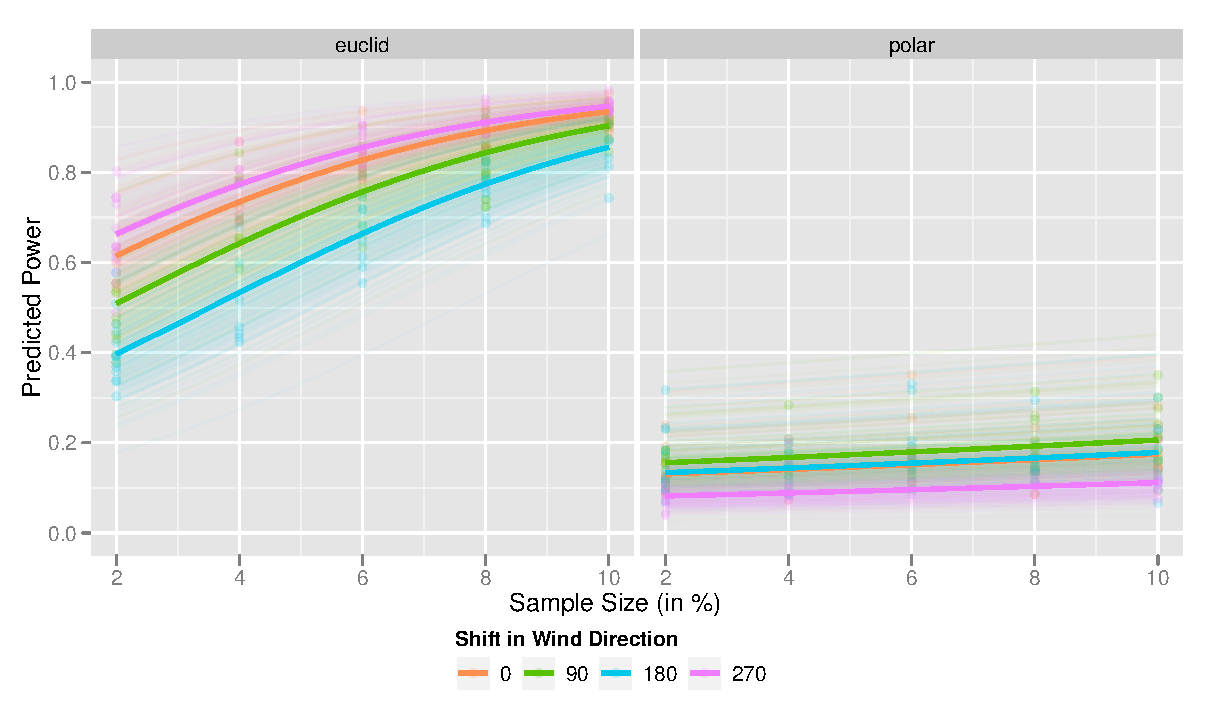
\includegraphics[width=\linewidth]{predict-power} 
   \caption{Predicted Power of designs.  The thin lines and the points on $y$ axis show  variability due to individuals' abilities. The saturated lines show average predicted power for each of the designs.}
   \label{fig:power}
\end{figure*}

The goal of this experiment is to understand the efficiency of displaying information using euclidian and polar coordinates. Efficiency is the deviation from independence, which can be simulated by taking permutations of the original dataset. Data concerning wind patterns and time between flights at SEA airport is used for these charts. The lineup chart is composed of 20 graphics with all of the exact same characteristics except for the data. One of the 20 graphics will be using original airport data while the other 19 will be permutations of that data. Efficiency of the chart types can be inferred by how accurately individuals pick out the plot with the original data. There are other variables which are introduced to further our understanding of the way we perceive euclidian and polar coordinates. All combinations of each level of the variables are involved in the experiment for both polar and euclidian coordinates. The graphics in each chart will all have exactly the same level of the variables with the only difference being the data. 

The other variables which are monitored are existence of reference line, placement of x-axis, and sample size. It is possible that one of the chart types benefits more from additional components such as reference lines. The polar and euclidian null charts will be shown either with or without a white reference line. The line is placed at slightly over 50 percent of the y axis. Additionally, the x-axis has four placements. The original dataset contains a characteristic wave pattern, which for euclidian coordinates, may be a large factor contributing to the perceived effectiveness of the graphic. Characteristic patterns such as the wave pattern may be perceived in a different way when viewed in polar coordinates. When the x-axis is is shifted the look of the pattern changes. The wave pattern is broken up for euclidian coordinates but for polar coordinates is only shifted around the axis. Finally, the amount of information necessary for detection as well as correctness is a measure for efficiency of the charts so the sample size which was taken from the original dataset is of interest. The original data set contained XXX,XXX observations from which 2, 4, 6, 8, 10, and 24 percent of the observations were sampled. Small sample sizes are easier to obtain because of time and money constraints. It would be nice to know if there is one type of chart which can show data trends using less information. 


 All combinations of these variables were repeated for plots with a reference line and without a reference line, as shown in figure \ref{layouts}.This figure shows examples of graphics showing the actual data, which in the experiment would be randomly positioned among 19 null plots. In total there are XXX unique charts which represent all different combinations of sample size, coordinate type, x-axis placement, and whether or not there is a reference line. The charts are all assigned a difficulty level, which is based on sample size, on a scale from zero to four. There are two plots assigned a difficulty level of zero. These two charts, one polar and one Euclidian, were made from computer generated data and intended to be at the level where an individual, if he or she is not purely guessing, should be able to find the correct plot. 


Amazon's Mechanical Turk is an online service in which individuals can request and perform simple tasks and surveys for money. Using Turk we were able to gather data on how people responded to the charts. Each person is shown a series of ten charts and asked to choose the graphic on each chart which they think is "different". They then identify, from a list of choices, why they chose this particular chart as well as how confident they are on a scale of one to five. Personal information such as age group, gender, and education is also collected on a voluntary basis. The amount of time it took the individual to answer is also recorded. This study allows us to make informed judgments about how the plot type effects efficiency in terms of accuracy and time spent reading the plots. Xcite stephen few?X

Effect is deviation from independence. Cannot be properly measured statistically except in highly aggregated situations, where the effect might be washed out.

%Most generally this experiment can be paralleled to the pie chart versus barchart discussion. The Euclidian coordinate plot is made up of bars *whose?* areas are colored proportionally according to the data. The polar coordinate plot is made up of pie slices which are also colored proportionally according to the data. Viewers of these charts will visually decode the areas of the bars and pie slices and make a judgement based on their decoding. How accurate this judgment is is left to be discussed. According to  \citet[page=40]{kosslyn:2006}, area is usually perceived as a function of what the actual area is. This function is the area raised to an exponent of approximately 0.8 and then multiplied by a constant. However, when bars are parallel, the relative height of these bars is perceived very accurately. From this information, one could infer that the Euclidian coordinate plot may gain efficiency based on the height of the colored bars. 


Pie versus Barchart discussion is pretty old: cite some of the literature:

From Stephen Few, perceptual edge:
	When a graph is made, quantitative and categorical information is encoded by a display method. Then the information is visually decoded. This visual perception is a vital link. No matter how clever the choice of the information, and no matter how technologically impressive the encoding, a visualization fails if the decoding fails. Some display methods lead to efficient, accurate decoding, and others lead to inefficient, inaccurate decoding. It is only through scientific study of visual perception that informed judgments can be made about display methods. (William S. Cleveland, The Elements of Graphing Data, Hobart Press, 1994, p. 1)
	
	The systematic distortion of area is captured by �Steven�s Power Law,� which states that the psychological impression is a function of the actual physical magnitude raised to an exponent (and multiplied by a scaling constant). To be precise, the perceived area is usually equal to the actual area raised to an exponent of about 0.8, times a scaling constant...In contrast, relative line length [such as the lengths of bars] is perceived almost perfectly, provided that the lines are oriented the same way \cite[page=40]{kosslyn:2006}
	
	
	We make angle judgments when we read a pie chart, but we don�t judge angles very well. These judgments are biased; we underestimate acute angles (angles less than 90�) and overestimate obtuse angles (angles greater than 90�). Also, angles with horizontal bisectors (when the line dividing the angle in two is horizontal) appear larger than angles with vertical bisectors. (Naomi Robbins, Creating More Effective Graphs, Wiley, 2005, p. 49)
	
	 Edward Tufte once said that �the only worse design than a pie chart is several of them, for then the viewer is asked to compare quantities located in spatial disarray both within and between pies� (Edward Tufte, The Visual Display of Quantitative Information, Graphics Press, 1983, p. 178.)

 We do not claim to settle the question - which is multi-facetted and will not have a clear 'winning' design but instead very much depends on the purpose of the chart and task at hand.


% !TEX root = comparison.tex
\subsection{Comparing Distribution Centers}

Since each participant provides results from nine lineups, we can use a generalized linear mixed effects model of power and account for individuals' abilities by including a subject-specific random intercept. We included all of the above described covariates  in the model, both as main effects and as two-way interaction with the design to assess their impact on the power of each of the designs.
Figure \ref{fig:power2} summarizes the modeling results as shown in table \ref{tbl:power2}. Generally we can see that the power of all four designs increases with an increase in effect size $d$ (on the $x$ axis), as well as an increasing sample size $n_1$ (top to bottom facetting). Generally, an increase of the second group also is beneficial to power. Unlike all of the other designs,  dotplots actually lose power significantly as the second group increases. 
The reason behind this phenomenon might be visual complexity: dotplots are the only design that show individuals. With an increase in group size, visual complexity increases with it, which could hamper the observer in evaluating shifts.

\begin{table}[ht]
\begin{center}
\resizebox{\linewidth}{!} {
\begin{tabular}{lrrrrrl}
  \hline
& & Estimate & Error & $t$-value & \multicolumn{2}{l}{approx $p$-value} \\   \hline
\\[-8pt]
\bf design& Intercept & -3.11 & 0.41 & -7.61 & 0.00 & ***\\ 
&  density & 0.05 & 0.57 & 0.09 & 0.93 \\ 
&  dotplot & 0.46 & 0.57 & 0.81 & 0.42\\ 
&  histogram & 0.06 & 0.58 & 0.11 & 0.91 \\ [2pt]
\multicolumn{2}{l}{\bf covariates}\\
&  d & 1.77 & 0.34 & 5.18 & 0.00 & ***\\ 
&  n1$_{100}$ & 1.84 & 0.19 & 9.73 & 0.00 & ***\\ 
&  ratio & 0.84 & 0.33 & 2.56 & 0.01 & **\\ 
\multicolumn{2}{l}{\bf interactions}\\
&  density:d & -0.60 & 0.47 & -1.27 & 0.20 \\ 
&  dotplot:d & 0.03 & 0.46 & 0.07 & 0.95  \\ 
&  histogram:d & -0.28 & 0.48 & -0.59 & 0.56 \\ [1pt]
&  density:n1$_{100}$ & -0.10 & 0.26 & -0.36 & 0.72\\ 
&  dotplot:n1$_{100}$ & -0.77 & 0.26 & -3.00 & 0.00 & ***\\ 
&  histogram:n1$_{100}$ & -0.69 & 0.26 & -2.64 & 0.01 & ** \\ [1pt]
&  density:ratio & -0.28 & 0.47 & -0.59 & 0.56 \\ 
&  dotplot:ratio & -1.01 & 0.46 & -2.19 & 0.03 & * \\ 
&  histogram:ratio & -0.28 & 0.47 & -0.59 & 0.55 \\ 
   \hline
\\[-5pt]
   \multicolumn{5}{l}{Signif. codes:  0 `***' 0.001 `**' 0.01 `*' 0.05 `.' 0.1}
\end{tabular}}
\end{center}
\caption{\label{tbl:power2}Results from a Generalized Linear Mixed Effects Model of power of a  lineup given design and all two-way interactions with effect size $d$, group size $n_1$, and ratio to second to first group size. 
Note that for all terms involving $n_1$ estimate and error are multiplied by a factor of 100. 
Reference group for all effects are boxplot designs. The model fit is based on 2513 lineup evaluations by 208 participants. }
\end{table}

The two highly summarized designs benefit the most from an increase in sample size: both density charts and boxplots profit significantly more than histograms and dotplots. This might, again, be a hint towards a trade-off between visual complexity and amount of information shown as the basis for making decisions. 


Table \ref{tbl:speed2} gives an overview of results from a linear model for (log) evaluation time of lineups. Subject-specific speed (due to spatial ability) are accounted for  including a random intercept. Structurally, the model is the same as before, i.e. we regard effect size $d$, size $n_1$ of the first group, and the ratio $n_2/n_1$ between group sizes both as main effects and in two-way interactions with the four competing designs. To make estimate sizes comparable, we have again multiplied all estimates and standard errors involving the group size $n_1$ by 100. This means that we need to interpret those  estimates as average change if the group size is increased by 100 elements. 

\begin{table}[ht]
\begin{center}
\resizebox{\linewidth}{!} {
\begin{tabular}{lrrrrrl}
  \hline
& & Estimate & Error & $t$-value & \multicolumn{2}{l}{approx $p$-value} \\   \hline
\\[-8pt]
\bf design& Intercept & 3.85 & 0.09 & 42.21 & 0.00 & ***\\ 
&  density & 0.01 & 0.12 & 0.07 & 0.94 \\ 
&  dotplot & 0.03 & 0.12 & 0.26 & 0.80 \\ 
&  histogram & 0.23 & 0.12 & 1.97 & 0.05 & . \\ [2pt]
\multicolumn{2}{l}{\bf covariates}\\
&      d & -0.23 & 0.08 & -3.02 & 0.00 & ***\\ [1pt]
&    n1$_{100}$ & 0.07 & 0.04 & 1.70 & 0.09 & .\\ [1pt]
&  ratio & -0.04 & 0.02 & -1.48 & 0.14  \\ [2pt]
\multicolumn{2}{l}{\bf interactions}\\
&  density:d & 0.11 & 0.11 & 1.02 & 0.31 \\ 
&  dotplot:d & 0.20 & 0.11 & 1.86 & 0.06 & .  \\ 
&  histogram:d & -0.01 & 0.11 & -0.09 & 0.93 \\ [1pt]
&  density:n1$_{100}$ & -0.12 & 0.06 & -2.11 & 0.03 & *\\ 
&  dotplot:n1$_{100}$ & -0.16 & 0.06 & -2.83 & 0.00 & ***\\ 
&  histogram:n1$_{100}$ & -0.05 & 0.06 & -0.93 & 0.35 \\ [1pt]
&  density:ratio & 0.04 & 0.03 & 1.18 & 0.24 \\ 
&  dotplot:ratio & 0.02 & 0.03 & 0.65 & 0.52 \\ 
&  histogram:ratio & 0.00 & 0.04 & 0.04 & 0.97 \\ 
   \hline
\\[-5pt]
   \multicolumn{5}{l}{Signif. codes:  0 `***' 0.001 `**' 0.01 `*' 0.05 `.' 0.1}
\end{tabular}}
\end{center}
\caption{\label{tbl:speed2}Results from a Linear Mixed Effects Model of (log) time to answer a lineup given design and all two-way interactions with effect size $d$, group size $n_1$, and ratio to second to first group size. Estimate and error for all terms involving $n_1$ are multiplied by a factor of 100 for comparability.
Reference group for all effects are boxplot designs. }
\end{table}

The results of this model are similar to the previous: evaluation speeds needed for the four different designs is very close, but  histograms take on average a significantly longer time ($e^{0.23} = 1.26$ seconds) to evaluate than lineups of boxplots. 
Where an increase of sample size led to an increase of accuracy before, we now see that it increases time for evaluation of boxplot slightly, but not significantly so. What is interesting is that evaluation time decreases significantly with an increase in sample size, particularly for dotplots, but also for density charts. This is counter-intuitive to our previous argument on dotplots being affected by visual complexity the most. It seems, that observers of dotplot lineups come to a conclusion faster as sample size increases, albeit more often to  the wrong conclusion. Rather than visual complexity, this might be indicative that over-plotting is problematic in dotplots. While we tried to accommodate for over-plotting by making use of alpha-blending and jittering, this might not have been sufficient for the large sample size.
 
\begin{figure}[htbp] %  figure placement: here, top, bottom, or page
   \centering
   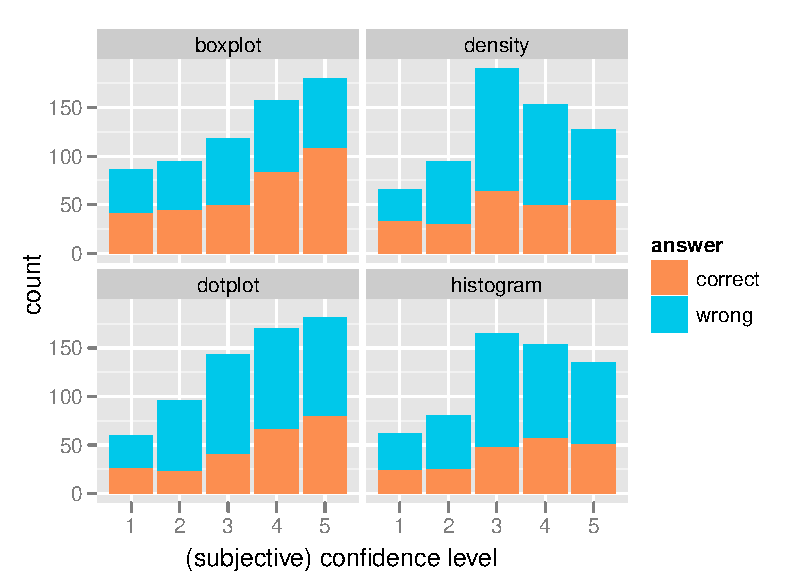
\includegraphics[width=\linewidth]{conf-exp2} 
   \caption{Barcharts of marginal distributions of self-reported confidence by design. The distributions display prominent differences.}
   \label{fig:conf-margins}
\end{figure}

Our third response variable is again the subjective assessment of confidence level. On average participants reported a confidence in their results of  3.41 (on a five point scale with 1=lowest and 5=highest), with a standard deviation of 0.149. Modeling confidence levels with a linear mixed effects model with the same structure as before resulted in only one significant effect beyond the intercept: participants report significantly higher confidence for increased number of  points in dotplot lineups. On average an increase of 100 points leads to an increase in confidence of 0.22 (with a standard error of 0.082). This finding is significant with a $p$-value of 0.007. 
Together with the previous results, we can tell that something worthy of further investigation happens in the perception of dotplots as sample sizes increase. 



Figure \ref{fig:conf-margins} shows barcharts of confidence assessments by design. It is obvious that the distribution of confidence is very different from one design to the next. Boxplots and dotplots show a similar pattern with an emphasis on high confidence levels, whereas histograms and density lineups have modes at a confidence level of three. 
One reason behind these differences in confidence distributions might be familiarity with the design - neither density charts nor histograms are particularly frequent displays for a general audience. 





% !TEX root = comparison.tex
\section{Results and Discussion}~\label{results}
%
\subsection{Wind Direction and Airport Efficiency}



Figures \ref{fig:time} and \ref{fig:conf} give an overview of the relationship between the three response variables: accuracy, speed, and confidence level.

Figure \ref{fig:time} shows histogram of the time participants needed to make a decision on each lineup. Correctness of answers is shown by color.  Because of the skewness of the distributions, times were log-transformed. Polar charts take on average more time to answer, and are answered with much lower accuracy. 
The average amount of time spent on a Euclidean lineup is $e^{3.53} = 34.1$ seconds compared to $e^{4.07}=58.5$ seconds for a polar lineup.
This is in stark contrast to accuracy: 76.92\% of the Euclidean lineups shown resulted in the a correct identification of the real data while only 20.31\% of the polar charts were correct.


\begin{figure}[hbtp] %  figure placement: here, top, bottom, or page
   \centering
   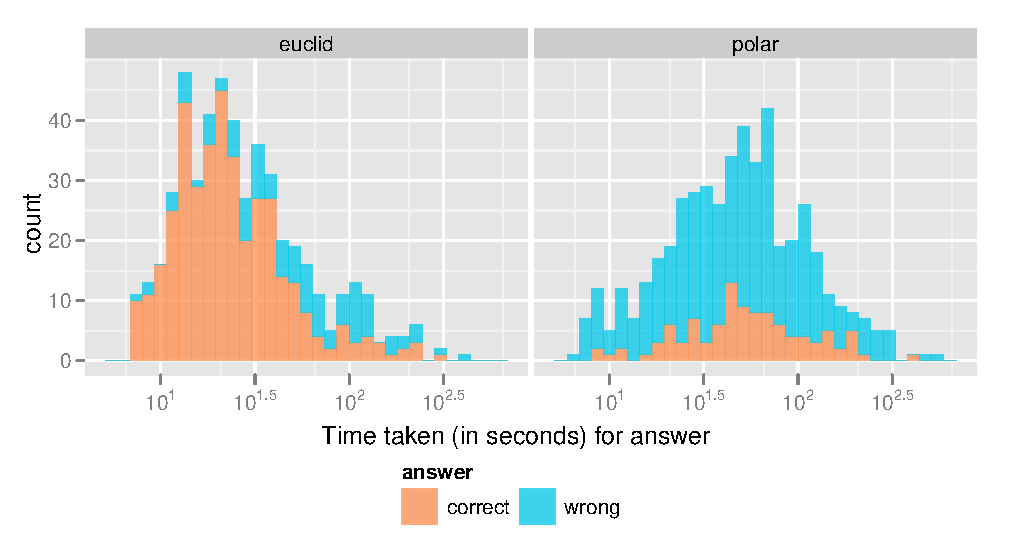
\includegraphics[width=\linewidth]{time-answer} 
   \caption{Histograms of time taken for answering lineups. On average the Euclidean design is answered faster and with higher power (percentage of correct answers). }
   \label{fig:time}
\end{figure}

Figure \ref{fig:conf} shows two barcharts of confidence levels by task, again coloring is used for correctness of answers. Euclidean displays lead to a very bimodal distribution of confidence: participants are either very sure or not sure at all of their answer. Confidence levels in polar charts are distributed much more uniformly.
\begin{figure}[hbtp] %  figure placement: here, top, bottom, or page
   \centering
   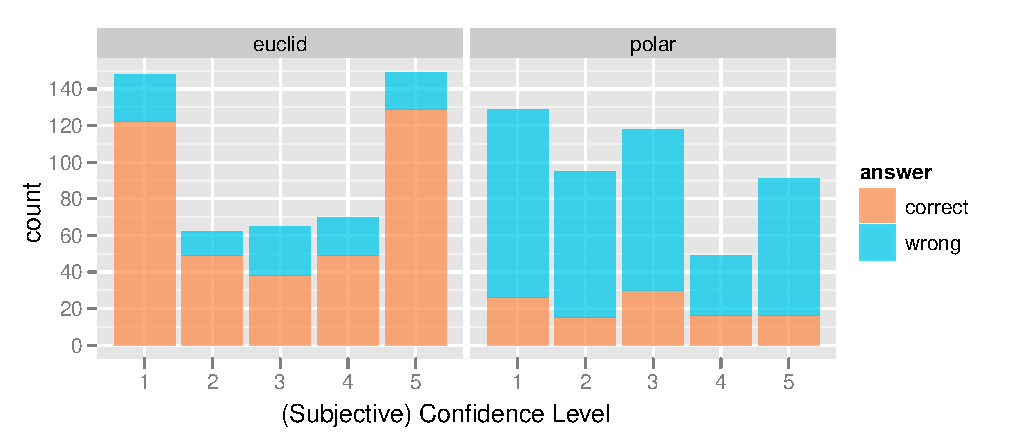
\includegraphics[width=\linewidth]{conf-answer} 
   \caption{Barcharts of self-reported confidence in answering correctly for each lineup. A strongly bimodal distribution is apparent, while confidence levels for polar charts are more uniform. Confidence levels are not indicative of accuracy: none of the differences between confidence levels show a significant difference in accuracy.}
   \label{fig:conf}
\end{figure}

The perceptual tasks involved in decoding the designs fit into the general framework of the piechart versus barchart discussion. However, we are not dealing with assessing angles, which is known to be perceptually harder than assessments of heights or widths in bars, see e.g. \cite{cleveland:1984, robbins:2004, Kosslyn:2006, few:2009}. Instead, the perceptual tasks consist of comparisons along a common axis (in the barcharts) and a common origin (in the polar charts). The difference in designs is therefore based on how well we are able to judge deviations from a horizontal line compared to deviations from a circle. Based on this, the charts with added reference lines provide us with exactly the frame we compare with and should, therefore, be the `better' designs - either in speed or accuracy.

Figure \ref{fig:treatment} shows a comparison of power for the four competing designs. 95\% confidence intervals are  Bonferroni adjusted for multiple testing. The bottom two confidence intervals in each panel show a 95\% confidence interval of a direct comparison of the Euclidean design versus the polar design with and without a reference line. With the exception of the 2\% sample none of those confidence intervals include the zero, indicating a significantly higher power for the Euclidean design than for the polar design.

\begin{figure}[htbp] %  figure placement: here, top, bottom, or page
   \centering

\begin{tabular}{cl}
\phantom{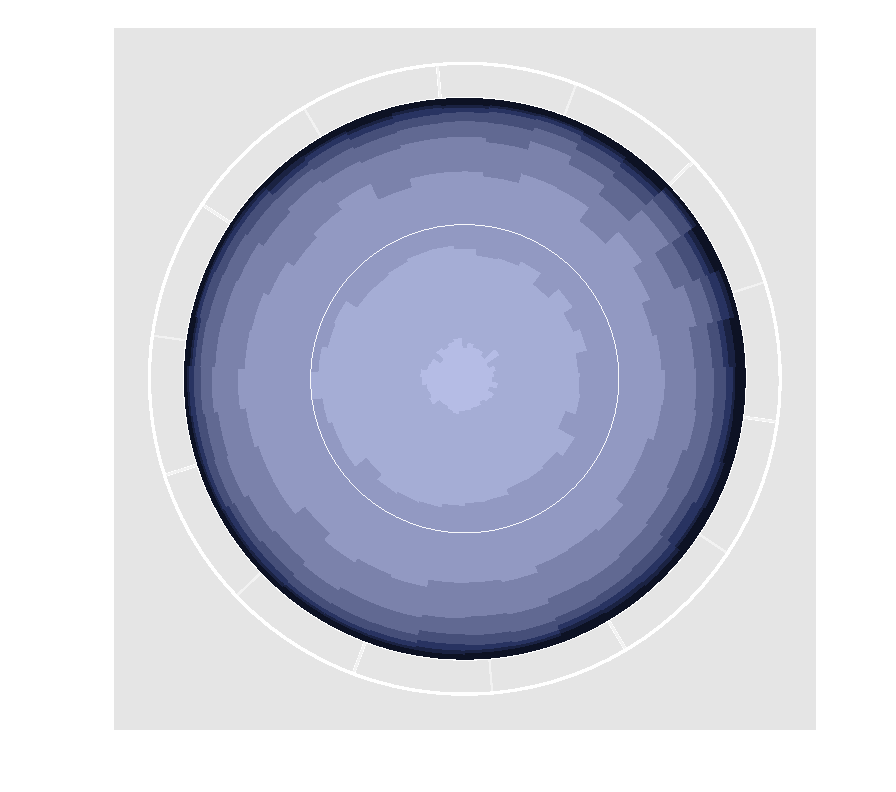
\includegraphics[width=0.03\linewidth]{Polar_Line.pdf}} & \vspace{-0.035in} \multirow{10}{*}{\hspace{-0.5in}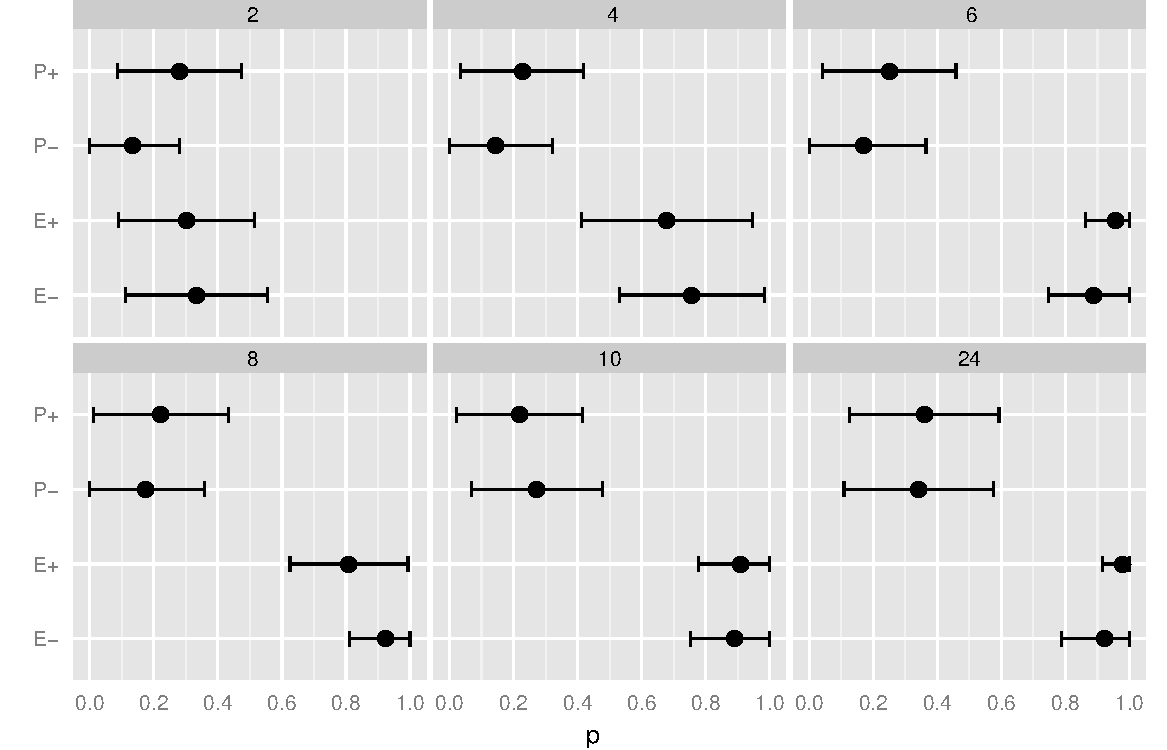
\includegraphics[width=0.9\linewidth]{turk4-designs.pdf}} \\
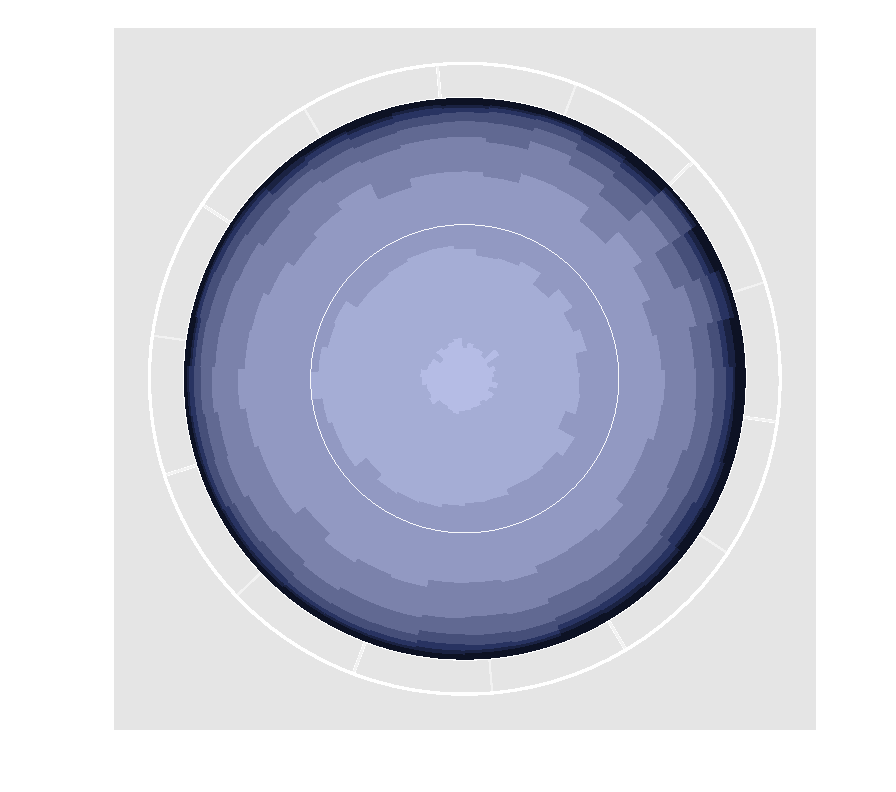
\includegraphics[width=0.045\linewidth]{Polar_Line.pdf} \\
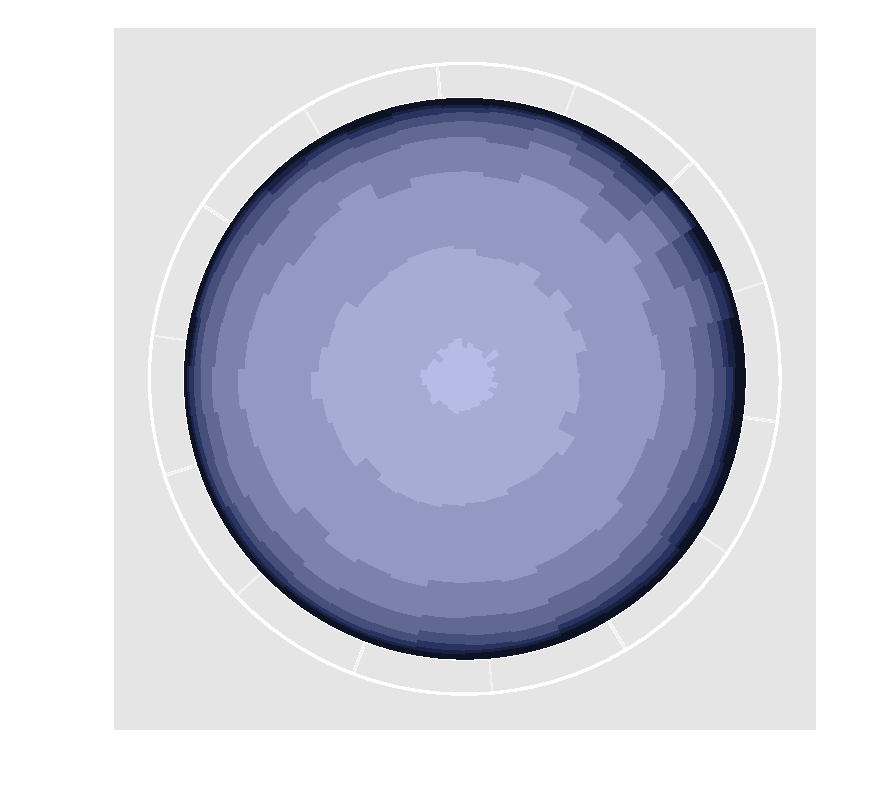
\includegraphics[width=0.045\linewidth]{Polar_NoLine.pdf} \\
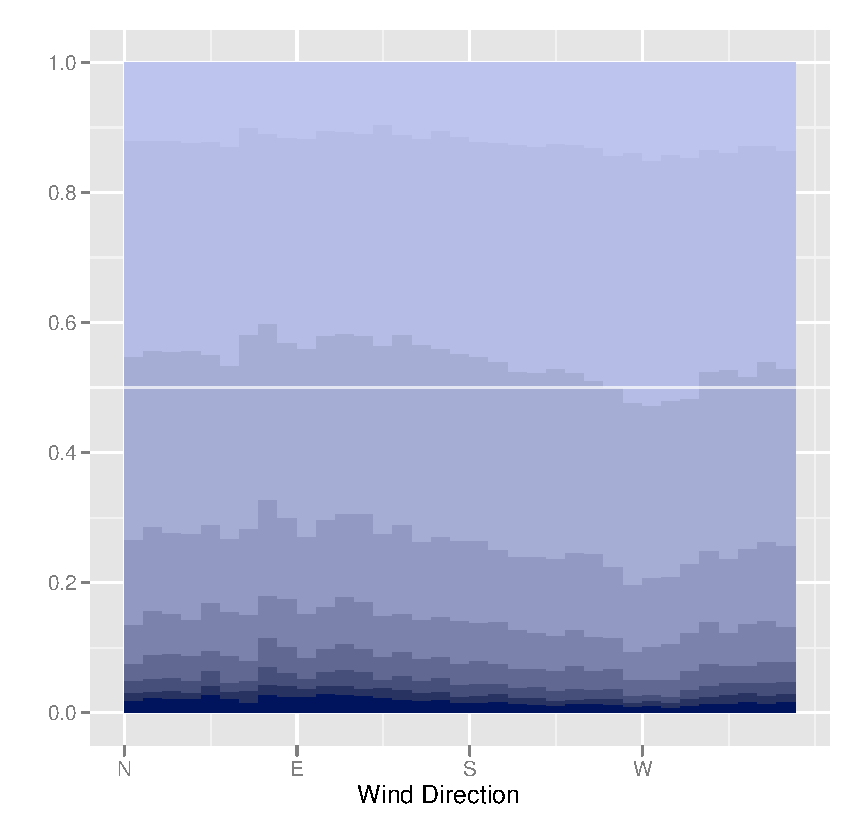
\includegraphics[width=0.043\linewidth]{Euclidian_Line.pdf} \\
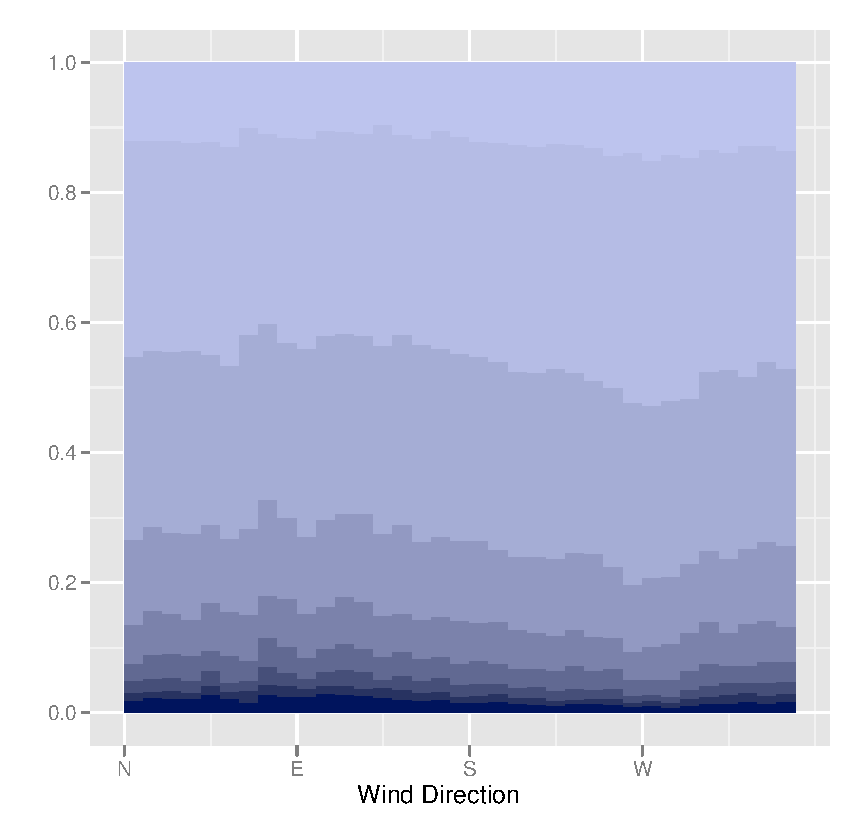
\includegraphics[width=0.043\linewidth]{Euclidian_NoLine.pdf}\\
\phantom{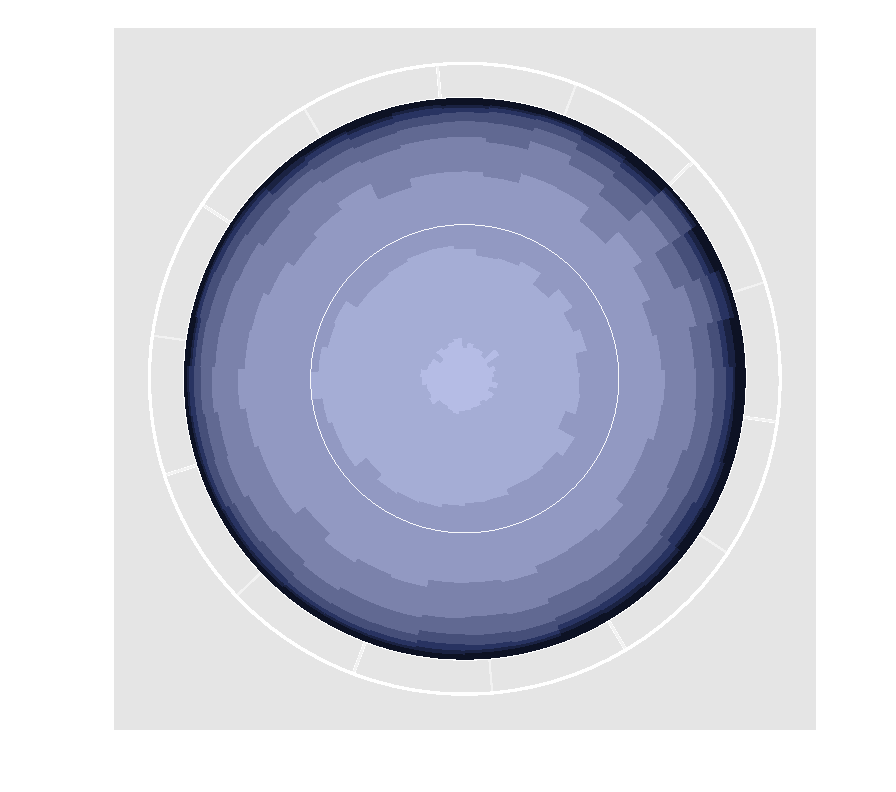
\includegraphics[width=0.13\linewidth]{Polar_Line.pdf}}\\
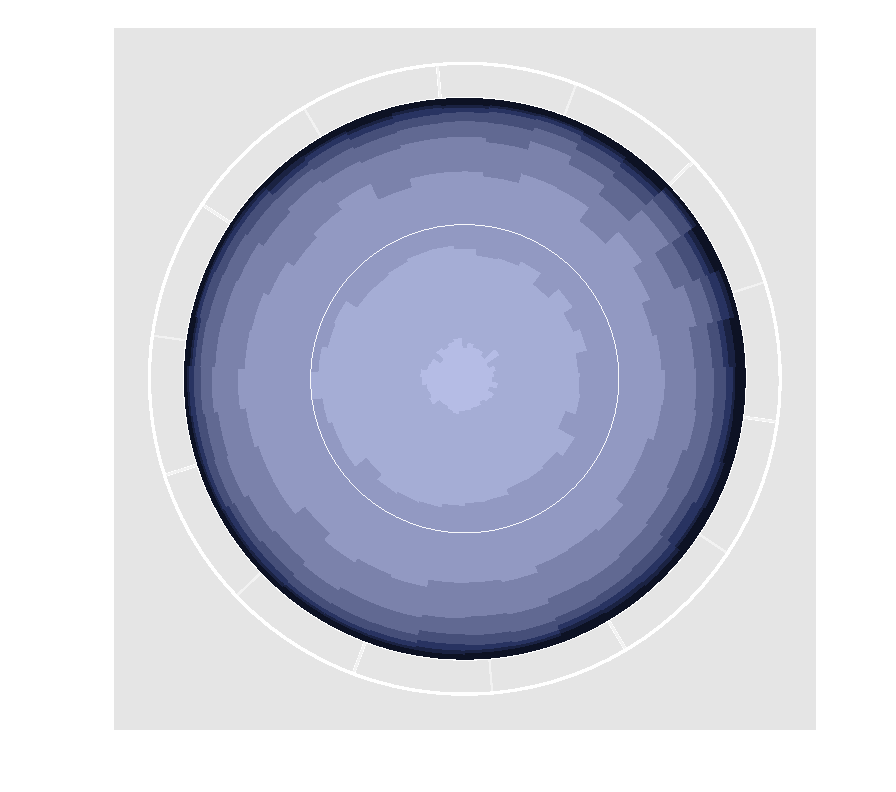
\includegraphics[width=0.045\linewidth]{Polar_Line.pdf} \\
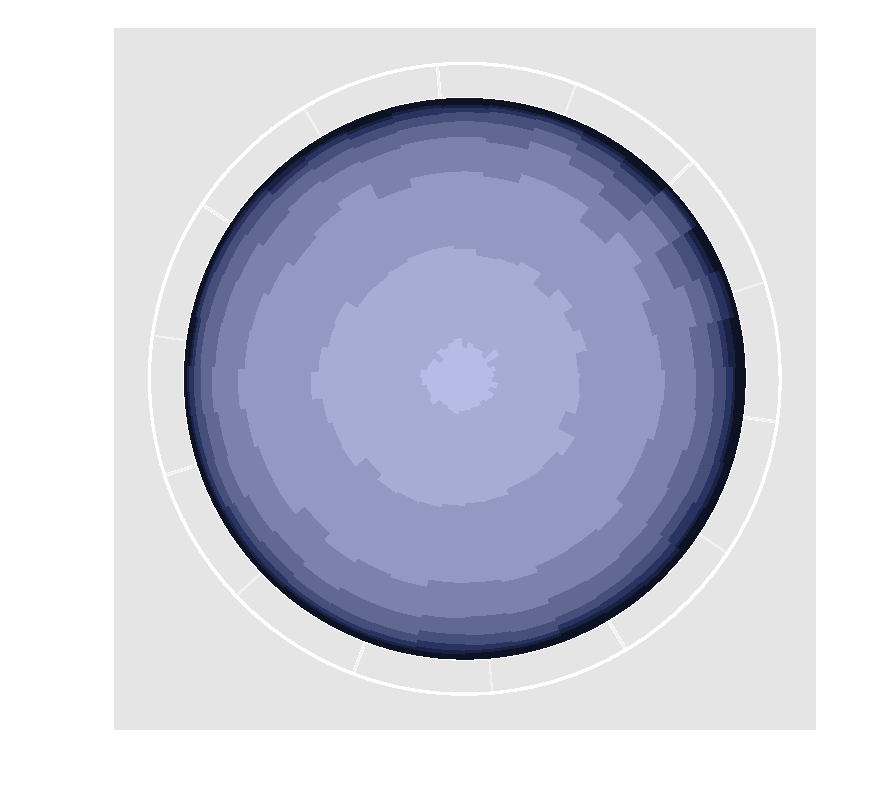
\includegraphics[width=0.045\linewidth]{Polar_NoLine.pdf} \\
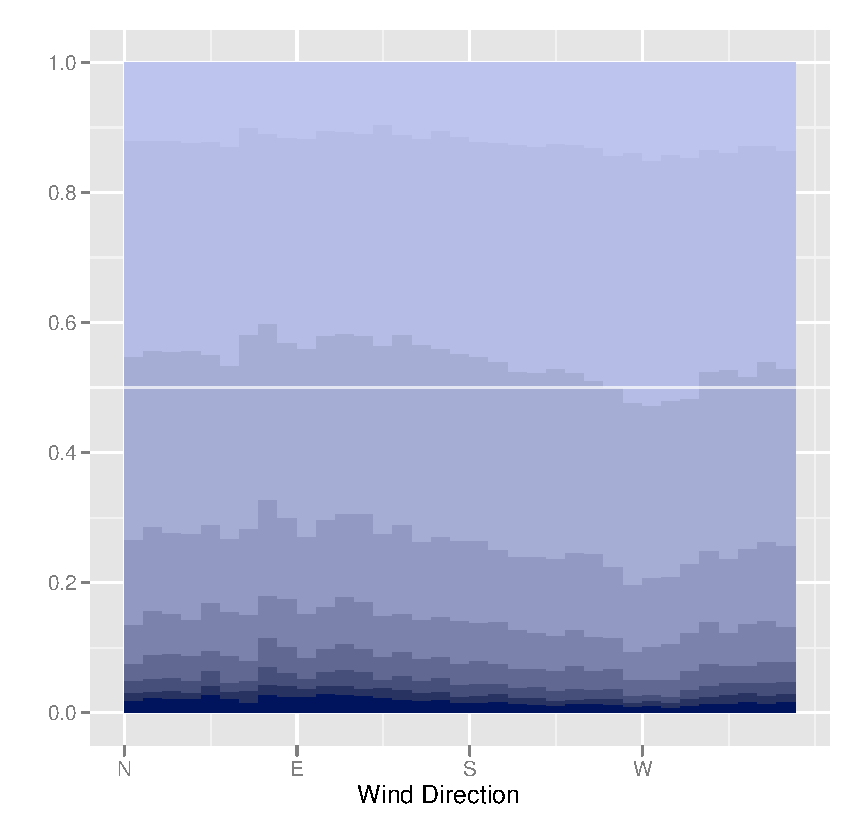
\includegraphics[width=0.043\linewidth]{Euclidian_Line.pdf} \\
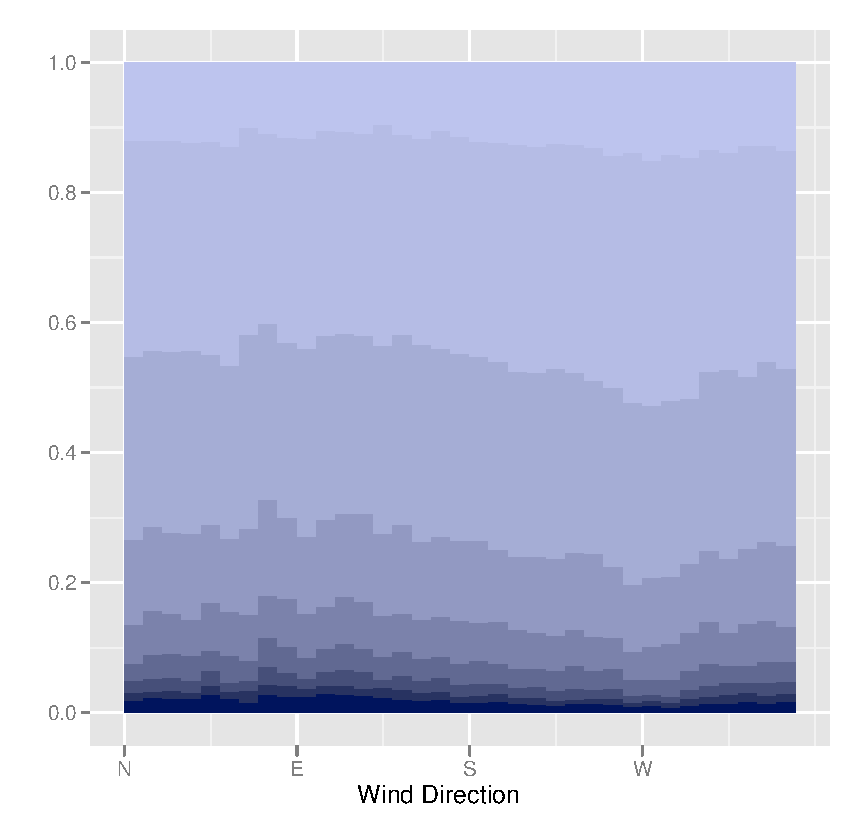
\includegraphics[width=0.043\linewidth]{Euclidian_NoLine.pdf}\\
\phantom{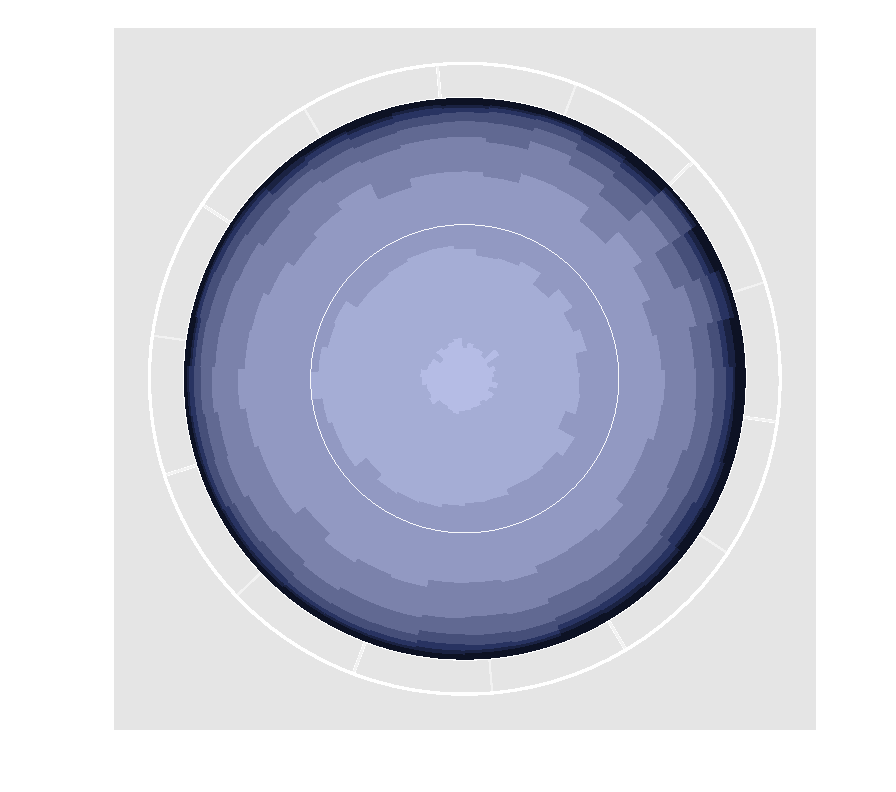
\includegraphics[width=0.13\linewidth]{Polar_Line.pdf}}\\
  \end{tabular} 
  \vspace{0.1in}
   \caption{Power results for two competing designs: polar versus  Euclidean, with and without a reference line; facetting indicates sample size (as percentage of original data). Error bars indicate single Bonferroni adjusted 95\% confidence intervals. The two confidence intervals at the bottom of each panel shows a pairwise power comparison of Euclidean versus polar design according to eqn (\ref{eq:comp}). Differences from zero (vertical grey line) are of interest.}
   \label{fig:treatment}
\end{figure}



%Most generally this experiment can be paralleled to the pie chart versus barchart discussion \cite{***}. 
%The Euclidean coordinate plot is made up of bars where areas are colored proportionally according to percentages. The polar coordinate plot is made up of pie slices which are also colored proportionally according to the data. 
%Viewers of these charts will visually decode the areas of the bars and pie slices and make a judgement based on their decoding. According to  \citet[page=40]{kosslyn:2006}, area is usually perceived as a function of what the actual area is. This function is the area raised to an exponent of approximately 0.8 and then multiplied by a constant. However, when bars are parallel, the relative height of these bars is perceived very accurately. From this information, one could infer that the Euclidean coordinate plot may gain efficiency based on the height of the colored bars. 


However, all of these considerations are based on the - rather strong - assumption that all individuals have the same ability to detect the data plot from a lineup. In order to allow for individual differences in visual ability, 
 we use a generalized linear mixed effects modeling  approach \cite{pinheiro:2000} for each of the three response values, using the {\tt R} package {\tt lme4} \cite{bates:2011}. 
For power predictions (cf. table \ref{tbl:correct}) a logistic regression was fitted for the competing designs, including covariates {\it sample size} (2, 4,6, 8, 10, and 24 percent of the data) and {\it shift} in wind direction (offset of 0, 90, 180, and 270 degrees), both as main effects and in two-way interaction effects with design to assess their effect on the power of designs. To adjust for individuals' ability, a random intercept was included in the model.

\begin{table}[ht]
\begin{center}
\resizebox{\linewidth}{!} {
%\rowcolors{2}{white}{lightgray}
\begin{tabular}{rrrrrrl}
  \hline
& & Estimate & Error & $z$-value & $p$-value &\\ 
  \hline
\bf design & euclid & -0.08 & 0.39 & -0.21 & 0.84 &\\ 
&polar & -1.98 & 0.32 & -6.13 & 0.00 & ***\\ [3pt]
\multicolumn{2}{l}{\bf main effects} &&&&&\\
& reference line  & -0.14 & 0.26 & -0.53 & 0.59 & \\ [1pt]
&  sample size & 0.27 & 0.04 & 6.31 & 0.00 & ***\\[1pt]
 &offset:  90 degrees& -0.43 & 0.37 & -1.18 & 0.24 &\\ 
  & 180 degrees& -0.89 & 0.35 & -2.51 & 0.01 & **\\ 
  & 270 degrees& 0.21 & 0.38 & 0.55 & 0.58 &\\ [3pt]
\multicolumn{2}{l}{\bf interactions} &&&&&\\
&  polar:line & 0.51 & 0.35 & 1.44 & 0.15 &\\ [1pt]
&    polar:sample size & -0.23 & 0.05 & -5.02 & 0.00 & ***\\[1pt]
&    polar:offset 90 & 0.64 & 0.49 & 1.30 & 0.20 \\ 
&  polar:offset 180 & 0.91 & 0.47 & 1.92 & 0.05 & .\\ 
&    polar:offset 270 & -0.73 & 0.54 & -1.35 & 0.18 &\\
   \hline
\\[-5pt]
   \multicolumn{5}{l}{Signif. codes:  0 `***' 0.001 `**' 0.01 `*' 0.05 `.' 0.1}
\end{tabular}
}
\end{center}
\caption{\label{tbl:correct} Output of a generalized linear mixed effects model for power of lineups (i.e. probability of identifying the data plot) for comparing designs. Included are two-way interactions with sample size and shifts in wind direction (offset). Euclidean designs without a reference line at offset 0 are used as baseline.
 Results are based on  976 lineup evaluations by 115 participants. }
\end{table}

%Note that we excluded demographic information about individuals (i.e., age, gender and education level), as none of these covariates exhibited any significant relationship with accuracy while adding to model complexity. 


Overall, the results show huge differences in the power of designs between polar charts and Euclidean: Euclidean designs are significantly more powerful than polar charts, particularly so with small sample sizes. 
 The reference line has surprisingly little influence, but it helps more for  polar charts than for Euclidean charts,
An increase in sample size has a positive impact on power. Polar charts need a much bigger sample size to see an increase in power -- only at about 24\% of the original data do we see about the same power as for Euclidean charts of a sample size of 2\%.
The  changes in offset are significant -- interestingly, borderline behavior (90 and 270 degrees) does not show a difference between polar and Euclidean charts, whereas an inversion of the wave pattern (first up, then down), does show a difference. The power of Euclidean lineups suffers significantly  from this inversion whereas power of polar charts is unaffected. This is an unexpected finding, but is consistent throughout different lineups in the data. Figure \ref{fig:power} summarizes the results from the model: power predictions ($y$ axis) are shown by sample size ($x$ axis). The thick lines show average power by design for different shifts in wind direction. The thin lines represent power for individuals. What can be seen is the different impact of the offset by design: while  an offset of 270 degrees (the `mountain' pattern) has the highest power in Euclidean charts, it comes out worst in polar charts.

\begin{figure}[htbp] %  figure placement: here, top, bottom, or page
   \centering
   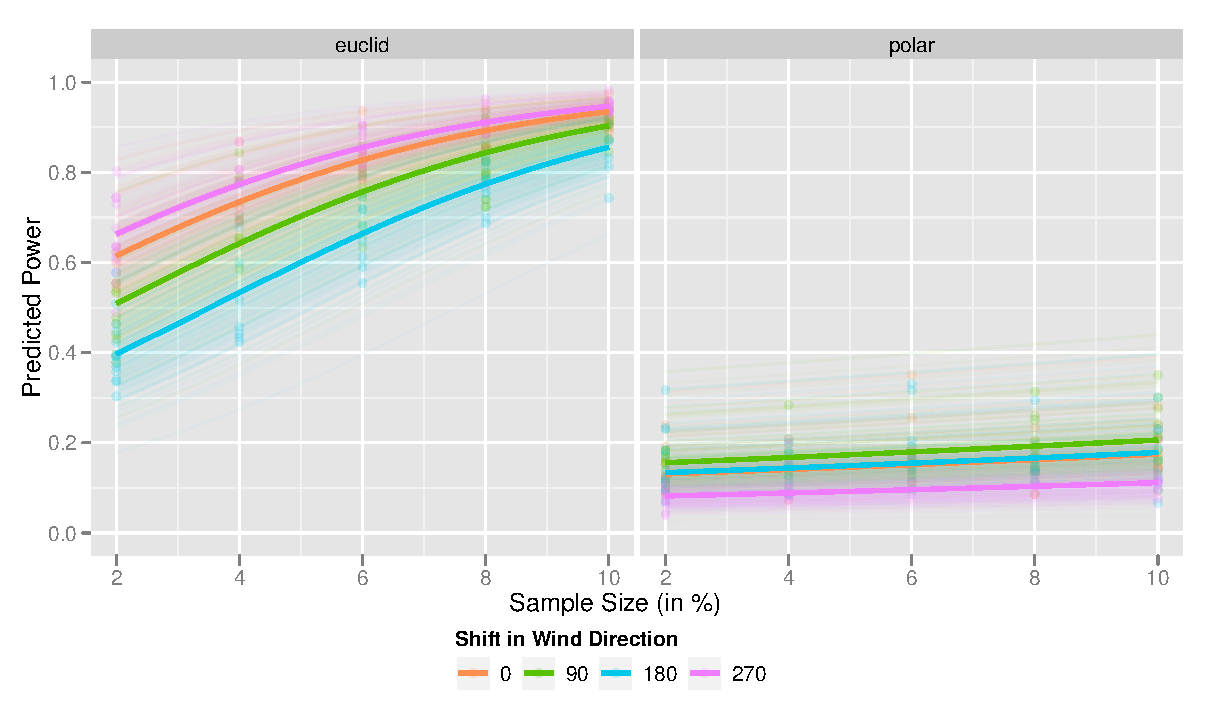
\includegraphics[width=\linewidth]{predict-power} 
   \caption{Predicted Power of designs.  The thin lines and the points on $y$ axis show  variability due to individuals' abilities. The saturated lines show average predicted power for each of the designs.}
   \label{fig:power}
\end{figure}

\begin{figure*}[hbtp] %  figure placement: here, top, bottom, or page
   \centering
   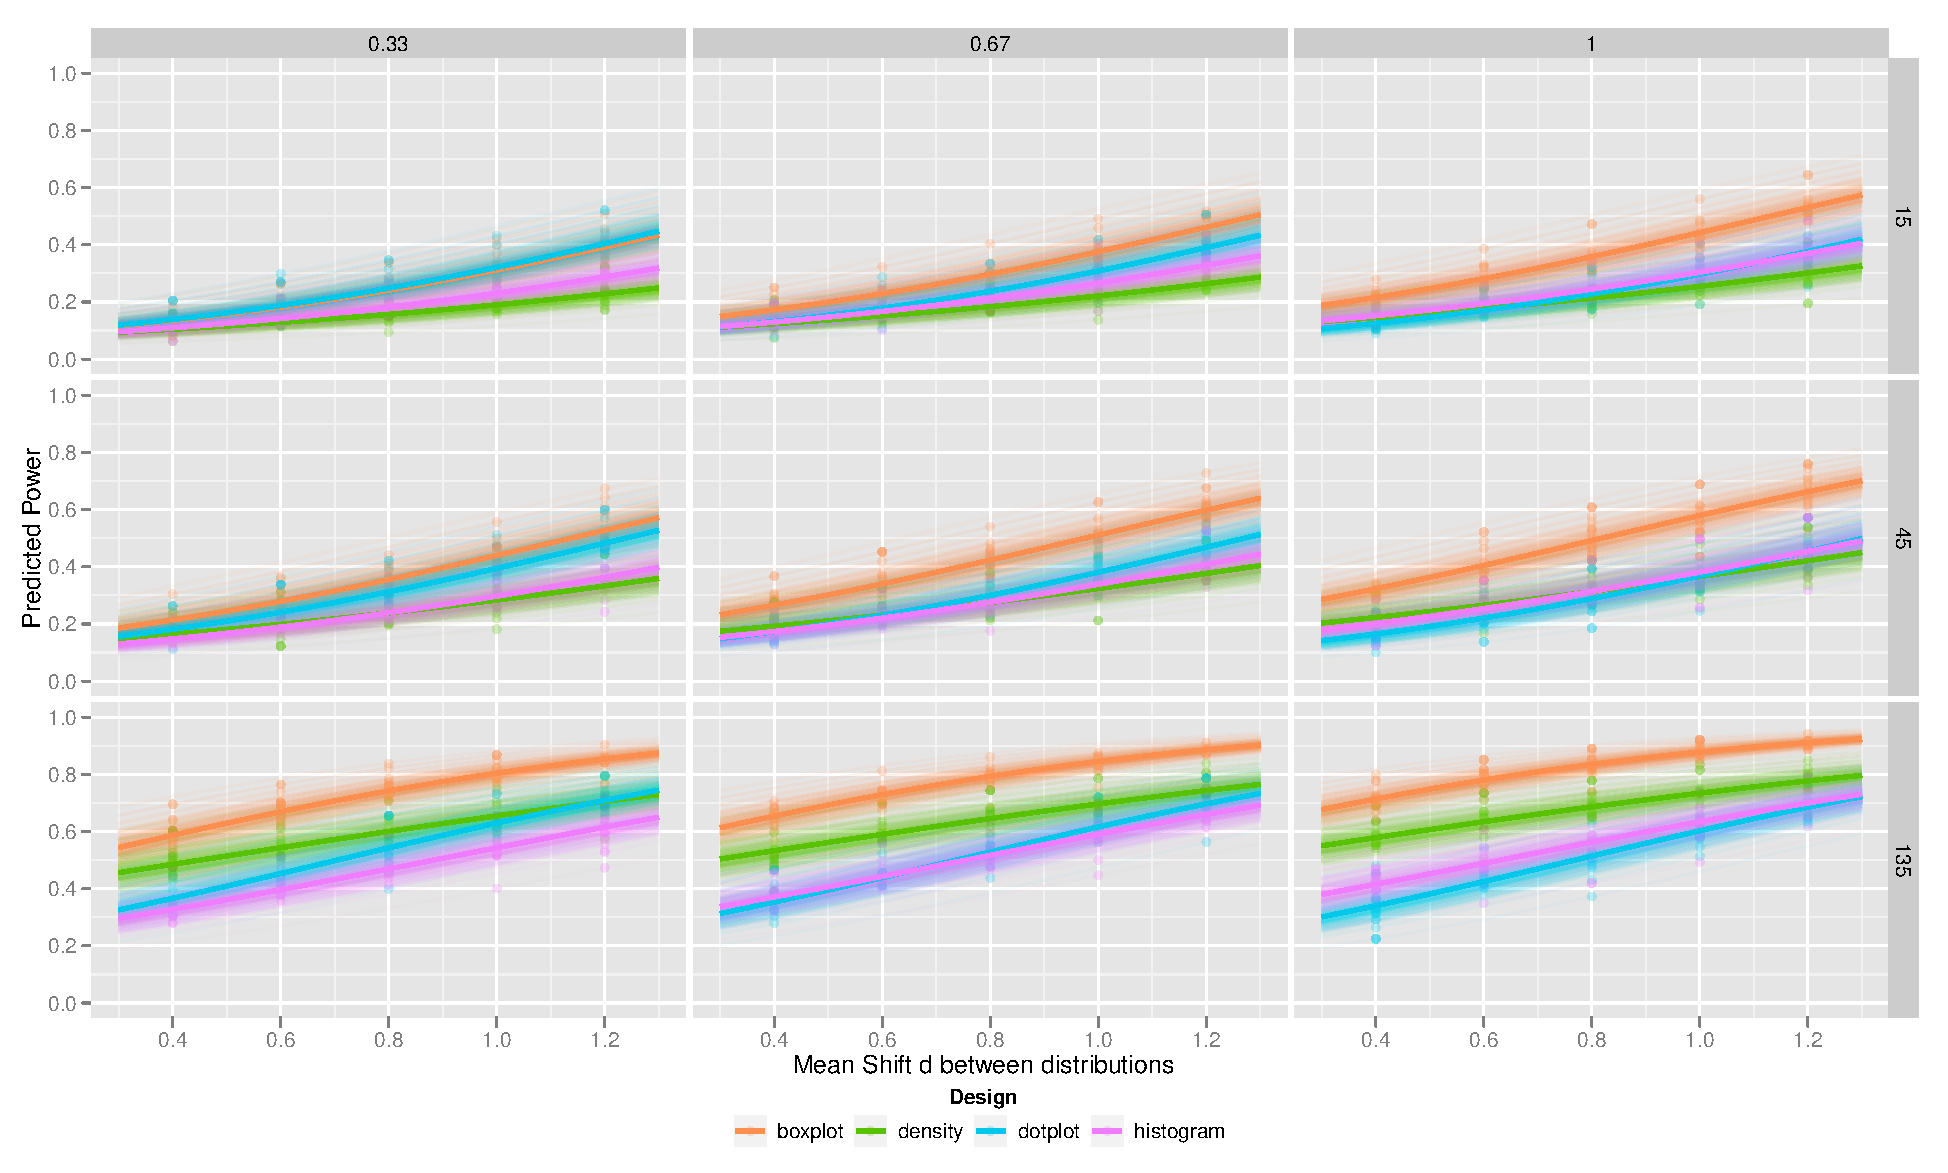
\includegraphics[width=0.9\linewidth]{power-exp2} 
   \caption{Overview of power predictions for the four different designs. The fully saturated thick lines show average predicted power for each of the designs facetted by size of the red group (top to bottom) and relative size of the blue group to the red group (left to right). Thin lines represent variability due to subject-specific abilities. }
   \label{fig:power2}
\end{figure*}

Time taken to answer was log transformed before the modeling process to de-emphasize the impact of very large values (up to 500 seconds). The findings are consistent with correctness - time taken shows big differences between polar and Euclidean charts. 
The reference lines seem to increase the evaluation time, but not significantly. An increase in sample size decreases evaluation time, The inversion of the wave pattern at 180 degrees leads to a significant increase in time for Euclidean charts, but not for polar charts (at least not significantly). Table \ref{tbl:time} shows an overview of the model parameters and estimates.

\begin{table}[ht]
\begin{center}
\resizebox{\linewidth}{!} {
%\rowcolors{2}{white}{lightgray}
\begin{tabular}{lrrrrrl}
  \hline
& & Estimate & Error & $t$-value & \multicolumn{2}{l}{approx $p$-value} \\   \hline
\bf design & Intercept & 3.58 & 0.09 & 41.34 & 0.00 & ***\\ 
&  polar & 0.22 & 0.10 & 2.17 & 0.03 & * \\ [2pt]
\multicolumn{2}{l}{\bf covariates}\\
&reference line & 0.08 & 0.06 & 1.50 & 0.13 \\ [1pt]
 & sample size & -0.03 & 0.00 & -8.73 & 0.00 & ***\\ [1pt]
&  offset: 90 & -0.06 & 0.08 & -0.72 & 0.47 \\ 
& 180 & 0.16 & 0.08 & 2.07 & 0.04 & *\\ 
&  270 & -0.04 & 0.07 & -0.54 & 0.59 \\ [2pt]
\multicolumn{2}{l}{\bf interactions}\\
&  polar:line & -0.03 & 0.08 & -0.40 & 0.69 \\ [1pt]
&    polar:sample size & 0.03 & 0.01 & 6.25 & 0.00 & ***\\ [1pt]
&    polar:offset 90 & 0.14 & 0.11 & 1.23 & 0.22 \\ 
&    polar:offset 180 & -0.17 & 0.11 & -1.55 & 0.12 \\ 
&    polar:offset 270 & 0.17 & 0.11 & 1.50 & 0.13 \\ 
   \hline
\\[-5pt]
   \multicolumn{5}{l}{Signif. codes:  0 `***' 0.001 `**' 0.01 `*' 0.05 `.' 0.1}
\end{tabular}}
\end{center}
\caption{\label{tbl:time} Model output for linear mixed effects model of (log) time taken, barchart design is baseline. }
\end{table}

 Confidence levels are measured on a five point scale --- they are subjective assessments by the participant `how certain are you'. We model confidence using the same model structure as before, i.e. using sample size and offset as covariates and including up to two-way interactions,
While there is a difference between the designs - participants reported higher confidence in dealing with the Euclidean lineups -- this is only  a trend (i.e. not significant at 5\% but below 10\%). The only significant effect on reported confidence level is the use of reference lines in polar coordinates: participants report an increase in confidence (0.31 $\pm$ 0.13, $p$ value = 0.01) when using the reference line. This, however, does not translate to a significant increase in accuracy of results, as we have seen before.

 Euclidean coordinates resulted in a significantly more accurate identification of the real data set in significantly shorter time.





%Euclidean coordinates performed better when speaking of efficiency in terms of accuracy and speed. 76.92\% of the Euclidean charts shown resulted in the a correct identification of the real data while only 20.31\% of the polar charts did the same. A t-test comparing means for charts with polar coordinates versus charts with Euclidean coordinates resulted in a t statistic of 15.2013 with a p-value of 2.2e-16. Similarly, a t-test comparing means of time spent on charts with Euclidean coordinates versus charts with polar coordinates resulted in a p-value of 1.014e-11. The average of the log of time spent on each individual chart for charts with Euclidean coordinates is 3.53 minutes while it was 4.07 minutes for charts with polar coordinates. Euclidean coordinates resulted in a significantly more accurate identification of the real data set in significantly shorter time. 

%\begin{figure}[htbp] %  figure placement: here, top, bottom, or page
%   \centering
%   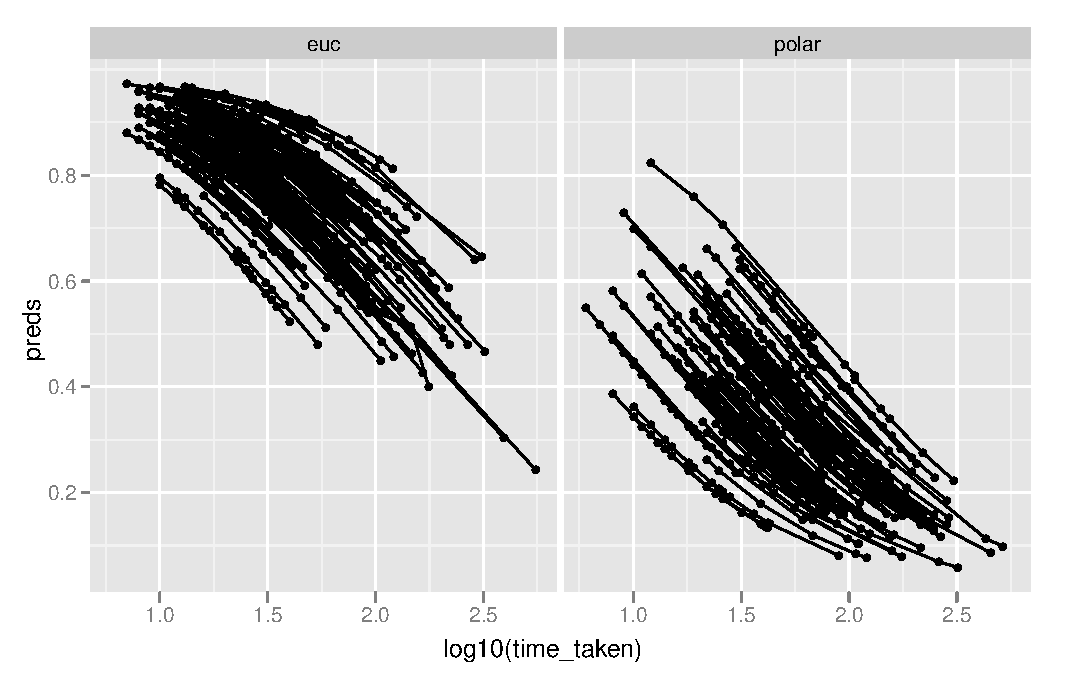
\includegraphics[width=3in]{turk4_time_perc_preds.pdf}  
%   \caption{Values predicted from XXXX how to say itXXXX of accuracy for log of time taken and test parameter.}
%   \label{accuracy_preds}
%\end{figure}
%
%Figure \ref{accuracy_preds} shows predicted accuracy levels. These predicted values were obtained by using R package lme4 and a mixed effect model explaining correct responses by type of chart and the log of time spent while accounting for different levels of accuracy for each individual who participated in the experiment. The predicted values show that there is an overall higher accuracy level for Euclidean coordinates when compared to polar coordinates. For both chart types, as the time spent increases, the predicted accuracy decreases. 
%
%\begin{figure}[htbp] %  figure placement: here, top, bottom, or page
%   \centering
%   %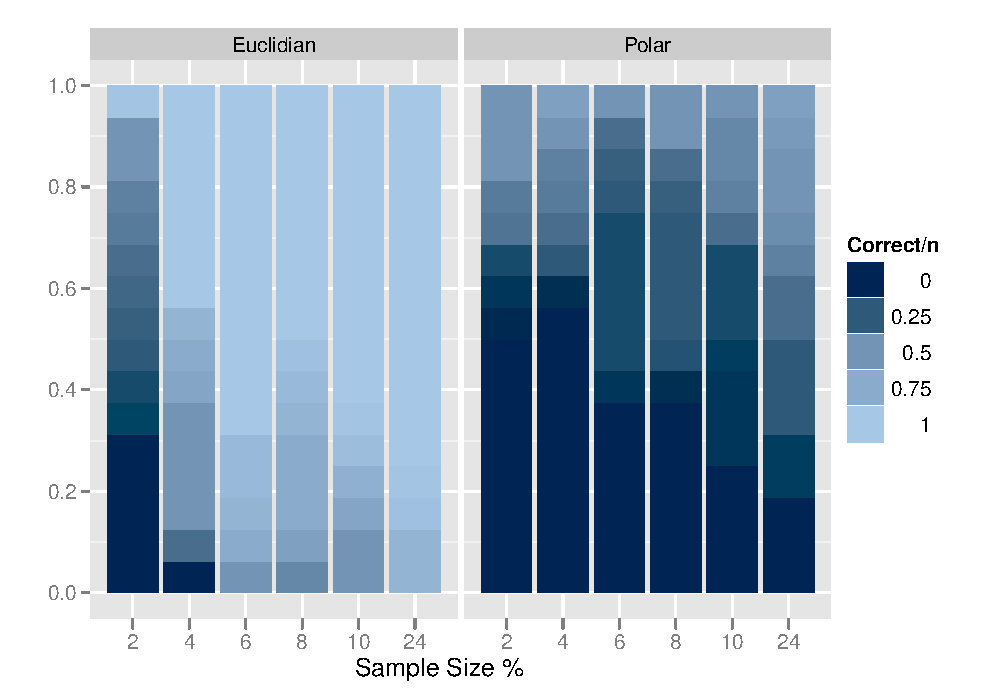
\includegraphics[width=3in]{turk4_samplesize_correctn.pdf}  
%   \caption{For each sample size for polar and Euclidean coordinates, the bars are colored according to the number of correct responses. Darker colors indicate lower accuracy levels while lighter colors indicate higher accuracy levels. }
%   \label{samp_size_acc}
%\end{figure}

%Ideally, efficient detection of data characteristics will be possible at small sample sizes. The difficulty of the charts is largely determined by the sample size taken from the original data set. Samples of 24 \% generally result in higher accuracy as the extra information facilitates detection of a relationship. Figure \ref{accuracy_preds} shows the relationship between the number of correct responses relative to the total number of responses and how this relationship differs between Euclidean and polar coordinates. The bars in the Euclidean plot are overall a lighter color than they are in the polar plot. This indicates a higher level of accuracy at all sample sizes. For Euclidean coordinates, we can see a stair step pattern in the accuracy levels as sample size increases. Lower levels of accuracy, indicated by darker colors, become consistently less prevalent as sample size increases. The relationship between sample size and accuracy level is not as simple for polar coordinates. Sample sizes of 2\% and 4\% have very similar accuracy levels. After 6\% the stair step pattern becomes visible and similar to that of Euclidean coordinates. Sample size seems to have less of an effect on accuracy for polar coordinates than it does for Euclidean coordinates. Predicted values of the proportion of correct responses when explained by sample size, the type of chart, and the interaction between these two factors, show that there is a significant difference between the relationship between sample size and correct responses for polar and Euclidean coordinates. Indeed, the proportion of correct responses increases more rapidly as sample size increases for Euclidean coordinates than it does for polar coordinates. 
%
%The effect of a reference line on accuracy and time was not statistically significant for both types of charts. When looking at plots of the data, however, the time spent on the charts seems to be higher when there is a reference line.This is true for both Euclidean and polar charts. Also visible in the data is a slight increase in accuracy with the presence of a reference line. These characteristics can be seen in figure\ref{reflines}.  
%
%\begin{figure}[htbp] %  figure placement: here, top, bottom, or page
%   \centering
%   %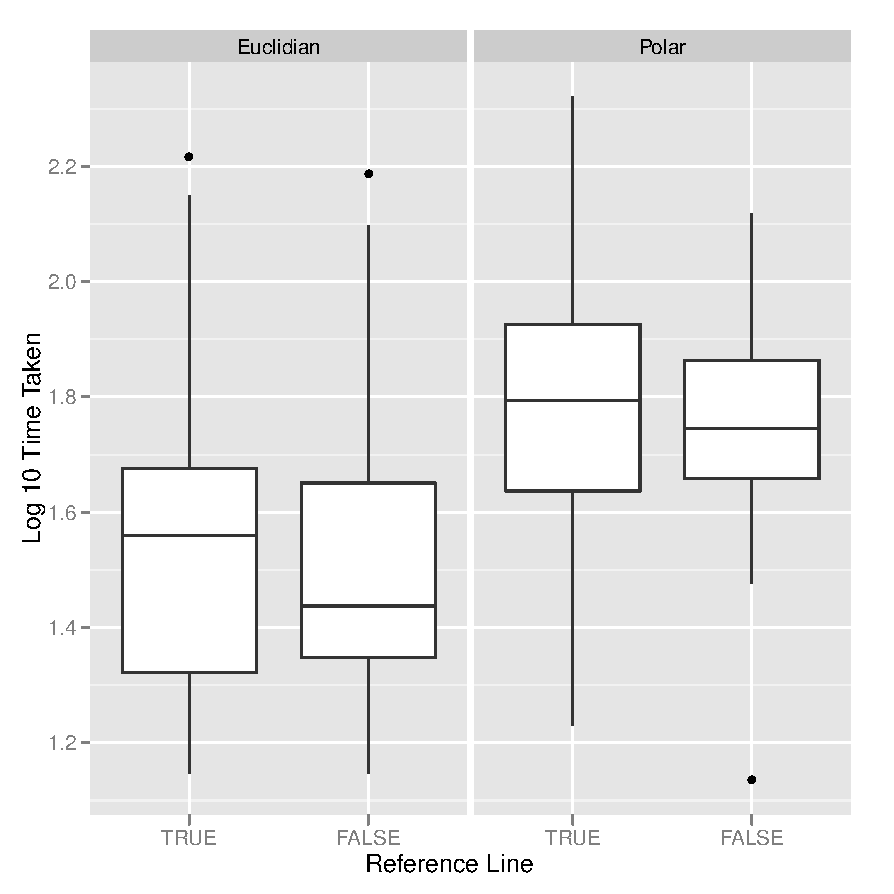
\includegraphics[width=1.5in]{turk4_refilne_time.pdf}  
%   %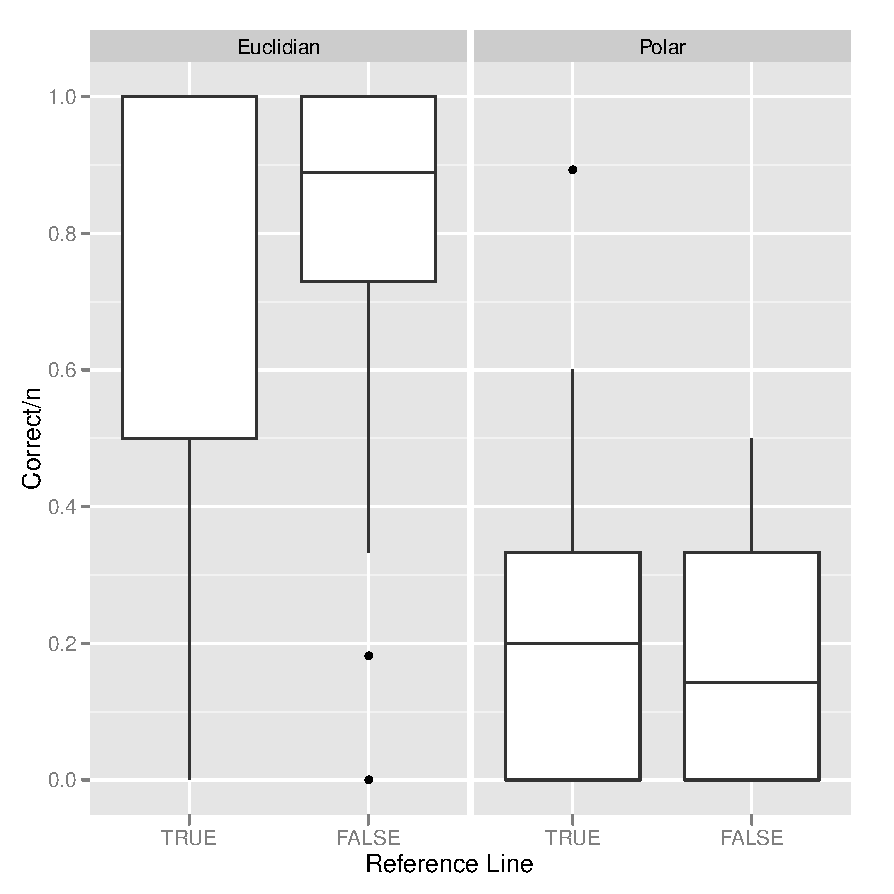
\includegraphics[width=1.5in]{turk4_refline_correctn.pdf}  
%   \caption{The relationship between reference line and time spent (left) and the relationship between reference line and accuracy (right). Although not statistically significant, some patterns are visible.}
%   \label{reflines}
%\end{figure}




\section{Conclusions}~\label{conclusions}

Could say something about adding a visual pleasure rating to the results, rate how attractive the display is on a scale of 1-5.



%% if specified like this the section will be ommitted in review mode
\acknowledgments{
This work was supported in part by
NSF DMS 1007697.}

\bibliographystyle{abbrv}
%%use following if all content of bibtex file should be shown
%\nocite{*}
\bibliography{references}
\end{document}